\appendix
\chapter{Dynamics of Merging Clusters Appendix}
\label{chap:dynamicsappendix}

\section{Potential Energy of Two Truncated NFW Halos}\label{potentialsec}

Generically the potential energy of a two-halo system with center to center separation $r$ is 
\begin{equation}
V(r) = \int \Phi_1(r') dm_2,
\label{potint}
\end{equation}
where $\Phi_1(r')$ is the gravitational potential of halo 1 as a function of radial distance $r'$ from the center of the halo 1 to the mass element of halo 2, $dm_2$.  
I derive $\Phi_1(r)$ for the case of a truncated NFW halo in \S \ref{nfwpotential}.
The integral of equation \ref{potint} can be approximated as a summation over $N \times N$ mass elements, $m_{2_{ij}}$, each with area $dr\times d\theta$, where $i$ and $j$ range from $0 \rightarrow N-1$,
\begin{displaymath}
V(r) \approx \sum_{i=0}^{N-1}\sum_{j=0}^{N-1} \Phi_1(r'_{ij}+\epsilon) m_{2_{ij}},
\end{displaymath}
where $r'_{ij}$ is the distance from the center of halo 1 to the 2$^{\rm nd}$ halo's mass element $m_{2_{ij}}$, as derived in \S\ref{masselements}, and $\epsilon$ is the softening length which reduces the effects of artificial singularities.

\subsection{Truncated NFW Gravitational Potential}\label{nfwpotential}

For an axially symmetric mass distribution the potential can be expressed as a series of Legendre Polynomials

\begin{equation}
\Phi_n(r) = -\frac{2\pi G}{(n+1/2)r^{n+1}} \int_{0}^{r} r'^{n+2} \rho_{n}(r')\,dr' -\frac{2\pi G r^n}{n+1/2} \int_{r}^{\infty} r'^{1-n} \rho_n(r')\,dr' 
\label{axsympot}
\end{equation}
where
\begin{equation}
\rho_n(r) = (n+1/2) \int_{0}^{\pi} \rho(r,\theta) P_n(\cos \theta) \sin \theta \,d\theta.
\label{lengden}
\end{equation}

Assuming a spherical NFW halo
\begin{displaymath}
\rho_{\rm NFW}(r) = \frac{\rho_s}{r/r_s(1+r/r_s)^2}
\end{displaymath}
only the zero$^{\rm th}$ order term of Equation \ref{lengden} remains
\begin{displaymath}
\rho_{\rm NFW}(r) = \rho_0(r)
\end{displaymath}
and Equation \ref{axsympot} reduces to
\begin{eqnarray}
\Phi_{\rm NFW}(r) & = & -\frac{4\pi G}{r}\int_{0}^{r} r'^2 \rho_{\rm NFW}(r')\,dr' - 4\pi G \int_{r}^{\infty}r' \rho_{\rm NFW}(r')\,dr' \nonumber\\
\Phi_{\rm NFW}(r) & = & -\frac{4\pi G \rho_s}{r} \left[ \int_{0}^{r} \frac{r'^2}{r'/r_s(1+r'/r_s)^2}\,dr' + r \int_{r}^{\infty} \frac{r'}{r'/r_s(1+r'/r_s)^2}\,dr' \right]. \nonumber
\end{eqnarray}
Since I truncate the NFW halo at $r_{200}$ the $\infty$ in the second integral becomes $r_{200}$ and
\begin{equation}
	\Phi_{\rm NFW_T}(r)=
	\begin{cases}
 		-\frac{4\pi G}{r} \rho_s r_s^3 \left[ \ln (1+r/r_s)-\frac{r}{r_s+r_{200}} \right], &\text{if $r\leq r_{200}$;}\\
  		-\frac{G M_{200}}{r}, &\text{if $r>r_{200}$.}
  	\end{cases}
\end{equation}

\subsection{Mass Elements of a Truncated NFW Halo}\label{masselements}

Given the differential mass elements for a spherically symmetric halo
\begin{displaymath}
dm = 2\pi\rho(r,\theta) r^2 \sin(\theta) d\theta\,dr,
\end{displaymath}
and discretizing the mass into elements with lengths $\delta r = r_{200_2}/N$ and $\delta\theta = \pi/N$ the halo 2 mass elements are given by
\begin{displaymath}
m_{ij} = 2\pi \int_{i\,\delta r}^{(i+1)\delta r} \int_{j\,\delta\theta}^{(j+1)\delta\theta} \rho(r') r'^2 \sin(\theta') d\theta'\,dr'.
\end{displaymath}
For an NFW halo this becomes
\begin{displaymath}
m_{ij} = 2\pi\rho_s r_s^3 \left[\cos(j\,\delta\theta)-\cos\left((j+1)\delta\theta\right) \right]\left[ \left( 1+\frac{(i+1)\delta r}{r_s}\right)^{-1} - \left(1+\frac{i\,\delta r}{r_s}\right)^{-1} + \ln\left[\frac{(i+1)\delta r+r_s}{i\,\delta r+r_s}\right]\right].
\end{displaymath}

\clearpage

\section{Musket Ball Cluster Redshift Catalog}\label{sec_MBCzcat}

The Musket Ball Cluster redshift catalog (Table \ref{table_MBCzcat}) contains 738 spectroscopically confirmed galaxy redshifts.  The galaxies are within an $\sim 18\arcmin \times 18\arcmin$ area centered on the Musket Ball Cluster ($139.05\deg$, $+29.85\deg$).  The source of the redshifts are from three separate spectroscopic surveys: 1) \emph{LRIS 2007} was carried out on 2007 January 15 using the Keck:I LRIS instrument, 2) \emph{DEIMOS 2011A} was carried out on 2011 March 1 \& 2 using the Keck:II DEIMOS instrument, and 3) \emph{DEIMOS 2012B} was carried out on 2013 January 16 using the Keck:II DEIMOS instrument.

The \emph{DEIMOS 2011A} observations consisted of 6 slit masks  with 1\arcsec slits and using the 1200\,line\,mm$^{-1}$ grating, tilted to a central wavelentgh of 6700\,\AA, resulting in a pixel scale of 0.33\,$\AA$\,pixel$^{-1}$, a resolution of $\sim1.1$\,\AA (50\,km\,s$^{-1}$), and typical wavelength coverage of 5400\AA\,to 8000\AA. 
The \emph{DEIMOS 2013B} observations consisted of 1 slit mask with 1\arcsec slits and using the 1200\,line\,mm$^{-1}$ grating, tilted to a central wavelentgh of 6200\,\AA, resulting in a pixel scale of 0.33\,\AA\,pixel$^{-1}$, a resolution of $\sim1$\,\AA (50\,km\,s$^{-1}$), and typical wavelength coverage of 4900\AA\,to 7500\AA. 
The exposures for each DEIMOS mask ($\sim3\times20$\,minutes) were combined using the DEEP2 version of the spec2d package \citep{Newman:2012ta}.
This package combines the individual exposures of the slit mosaic and performs wavelength calibration, cosmic ray removal and sky subtraction on slit-by-slit basis, generating a processed two-dimensional spectrum for each slit. 
The spec2d pipeline also generates a processed one-dimensional spectrum for each slit.
This extraction creates a one-dimensional spectrum of the target, containing the summed flux at each wavelength in an optimized window. 
Table \ref{table_MBCzcat} only includes high quality (Q $\geq$ 3, see \citet{Newman:2012ta} for an explanation on the quality codes) galaxy spectra.
Details of the \emph{LRIS 2007} observations and reduction are discussed in the Deep Lens Survey data release paper (Wittman et al. in prep).

%% The values (usually only l,r and c) in the last part of
%% \begin{deluxetable}{} command tell LaTeX how many columns
%% there are and how to align them.
\begin{deluxetable}{llcccccc}

%% Keep a portrait orientation

%% Over-ride the default font size
%% Use 8pt
\tabletypesize{\scriptsize}

%% Use \tablewidth{?pt} to over-ride the default table width.
%% If you are unhappy with the default look at the end of the
%% *.log file to see what the default was set at before adjusting
%% this value.
\tablewidth{0pt}

%% This is the title of the table.
\tablecaption{Musket Ball Cluster Redshift Catalog\label{table_MBCzcat}}

%% This command over-rides LaTeX's natural table count
%% and replaces it with this number.  LaTeX will increment
%% all other tables after this table based on this number
%\tablenum{4}

%% The \tablehead gives provides the column headers.  It
%% is currently set up so that the column labels are on the
%% top line and the units surrounded by ()s are in the
%% bottom line.  You may add more header information by writing
%% another line between these lines. For each column that requries
%% extra information be sure to include a \colhead{text} command
%% and remember to end any extra lines with \\ and include the
%% correct number of &s.
\tablehead{\colhead{RA} & \colhead{Dec} & \colhead{PosErr} & \colhead{z} & \colhead{$\sigma$z} & \colhead{Source} & \colhead{R } & \colhead{$\sigma$R} \\
\colhead{(hh:mm:ss.sss)} & \colhead{(dd:mm:ss.ss)} & \colhead{(arcsec)} & \colhead{} & \colhead{} & \colhead{} & \colhead{(mag)} & \colhead{(mag)} }
%% All data must appear between the \startdata and \enddata commands
\startdata
09:15:40.142 & +29:55:06.71 & 0.5 & 0.234777 & 0.000020 & DEIMOS 2011A & 20.983 & 0.007 \\
09:15:41.501 & +29:47:07.64 & 0.5 & 0.530381 & 0.000024 & DEIMOS 2011A & 23.398 & 0.048 \\
09:15:41.682 & +29:55:13.05 & 0.5 & 0.704062 & 0.000033 & DEIMOS 2011A & 22.586 & 0.024 \\
09:15:41.726 & +29:56:12.79 & 0.5 & 0.498200 & 0.000015 & DEIMOS 2011A & 22.664 & 0.016 \\
09:15:42.418 & +29:46:55.71 & 0.5 & 0.899342 & 0.000101 & DEIMOS 2011A & 22.246 & 0.017 \\
\enddata
%% Include any \tablenotetext{key}{text}, \tablerefs{ref list},
%% or \tablecomments{text} between the \enddata and
%% \end{deluxetable} commands

%% General table comment marker
\tablecomments{Table \ref{table_MBCzcat} is published in its entirety in the electronic
edition of the {\it Astrophysical Journal}.  A portion is shown here
for guidance regarding its form and content.}

%% No \tablerefs indicated

\end{deluxetable}

\clearpage

\section{Bullet Cluster Result Plots}\label{sec_bcresults}

This section contains the parameter results array plots for the Bullet Cluster case including the added temporal prior of \S\ref{sec_addedprior}.
For ease of display the parameters are grouped in three categories (\emph{Input}, \emph{Geometry}, and \emph{Velocity \& Time}) resulting in a six subplot results array, see Figure \ref{fig_resultsarray}.
The \emph{Input} parameters consist of: M$_{200_1}$, M$_{200_2}$, $z_1$, $z_2$,	and $d_{\rm proj}$, where halo 1 refers to the ``main'' subcluster and halo 2 refers to the ``bullet'' subcluster.
The \emph{Geometry} parameters consist of the randomly drawn $\alpha$, and calculated $d_{\rm 3D}$, and $d_{\rm max}$.
The calculated \emph{Velocity \& Time} parameters consist of:  $TSC_0$, $TSC_1$, and $T$.

\begin{figure}[b]
\centering
\includegraphics[width=6in]{Appendix1/ResultsArray_RevB.png}
\caption[Dynamics results array configuration.]{
For ease of display the results array is divided into six subplots, Figures \ref{fig_bc_inin}--\ref{fig_bc_geovt}.
The Input parameters consist of: M$_{200_1}$, M$_{200_2}$, $z_1$, $z_2$,	and $d_{\rm proj}$.
The calculated Geometry parameters consist of: $\alpha$, $d_{\rm 3D}$, and $d_{\rm max}$.
The calculated Velocity \& Time parameters consist of:  $v_{\rm 3D}(t_{\rm obs})$, $v_{\rm 3D}(t_{\rm col})$, $TSC_0$, $TSC_1$, and $T$.
\label{fig_resultsarray}}
\end{figure}
\clearpage

\begin{figure}
\centering
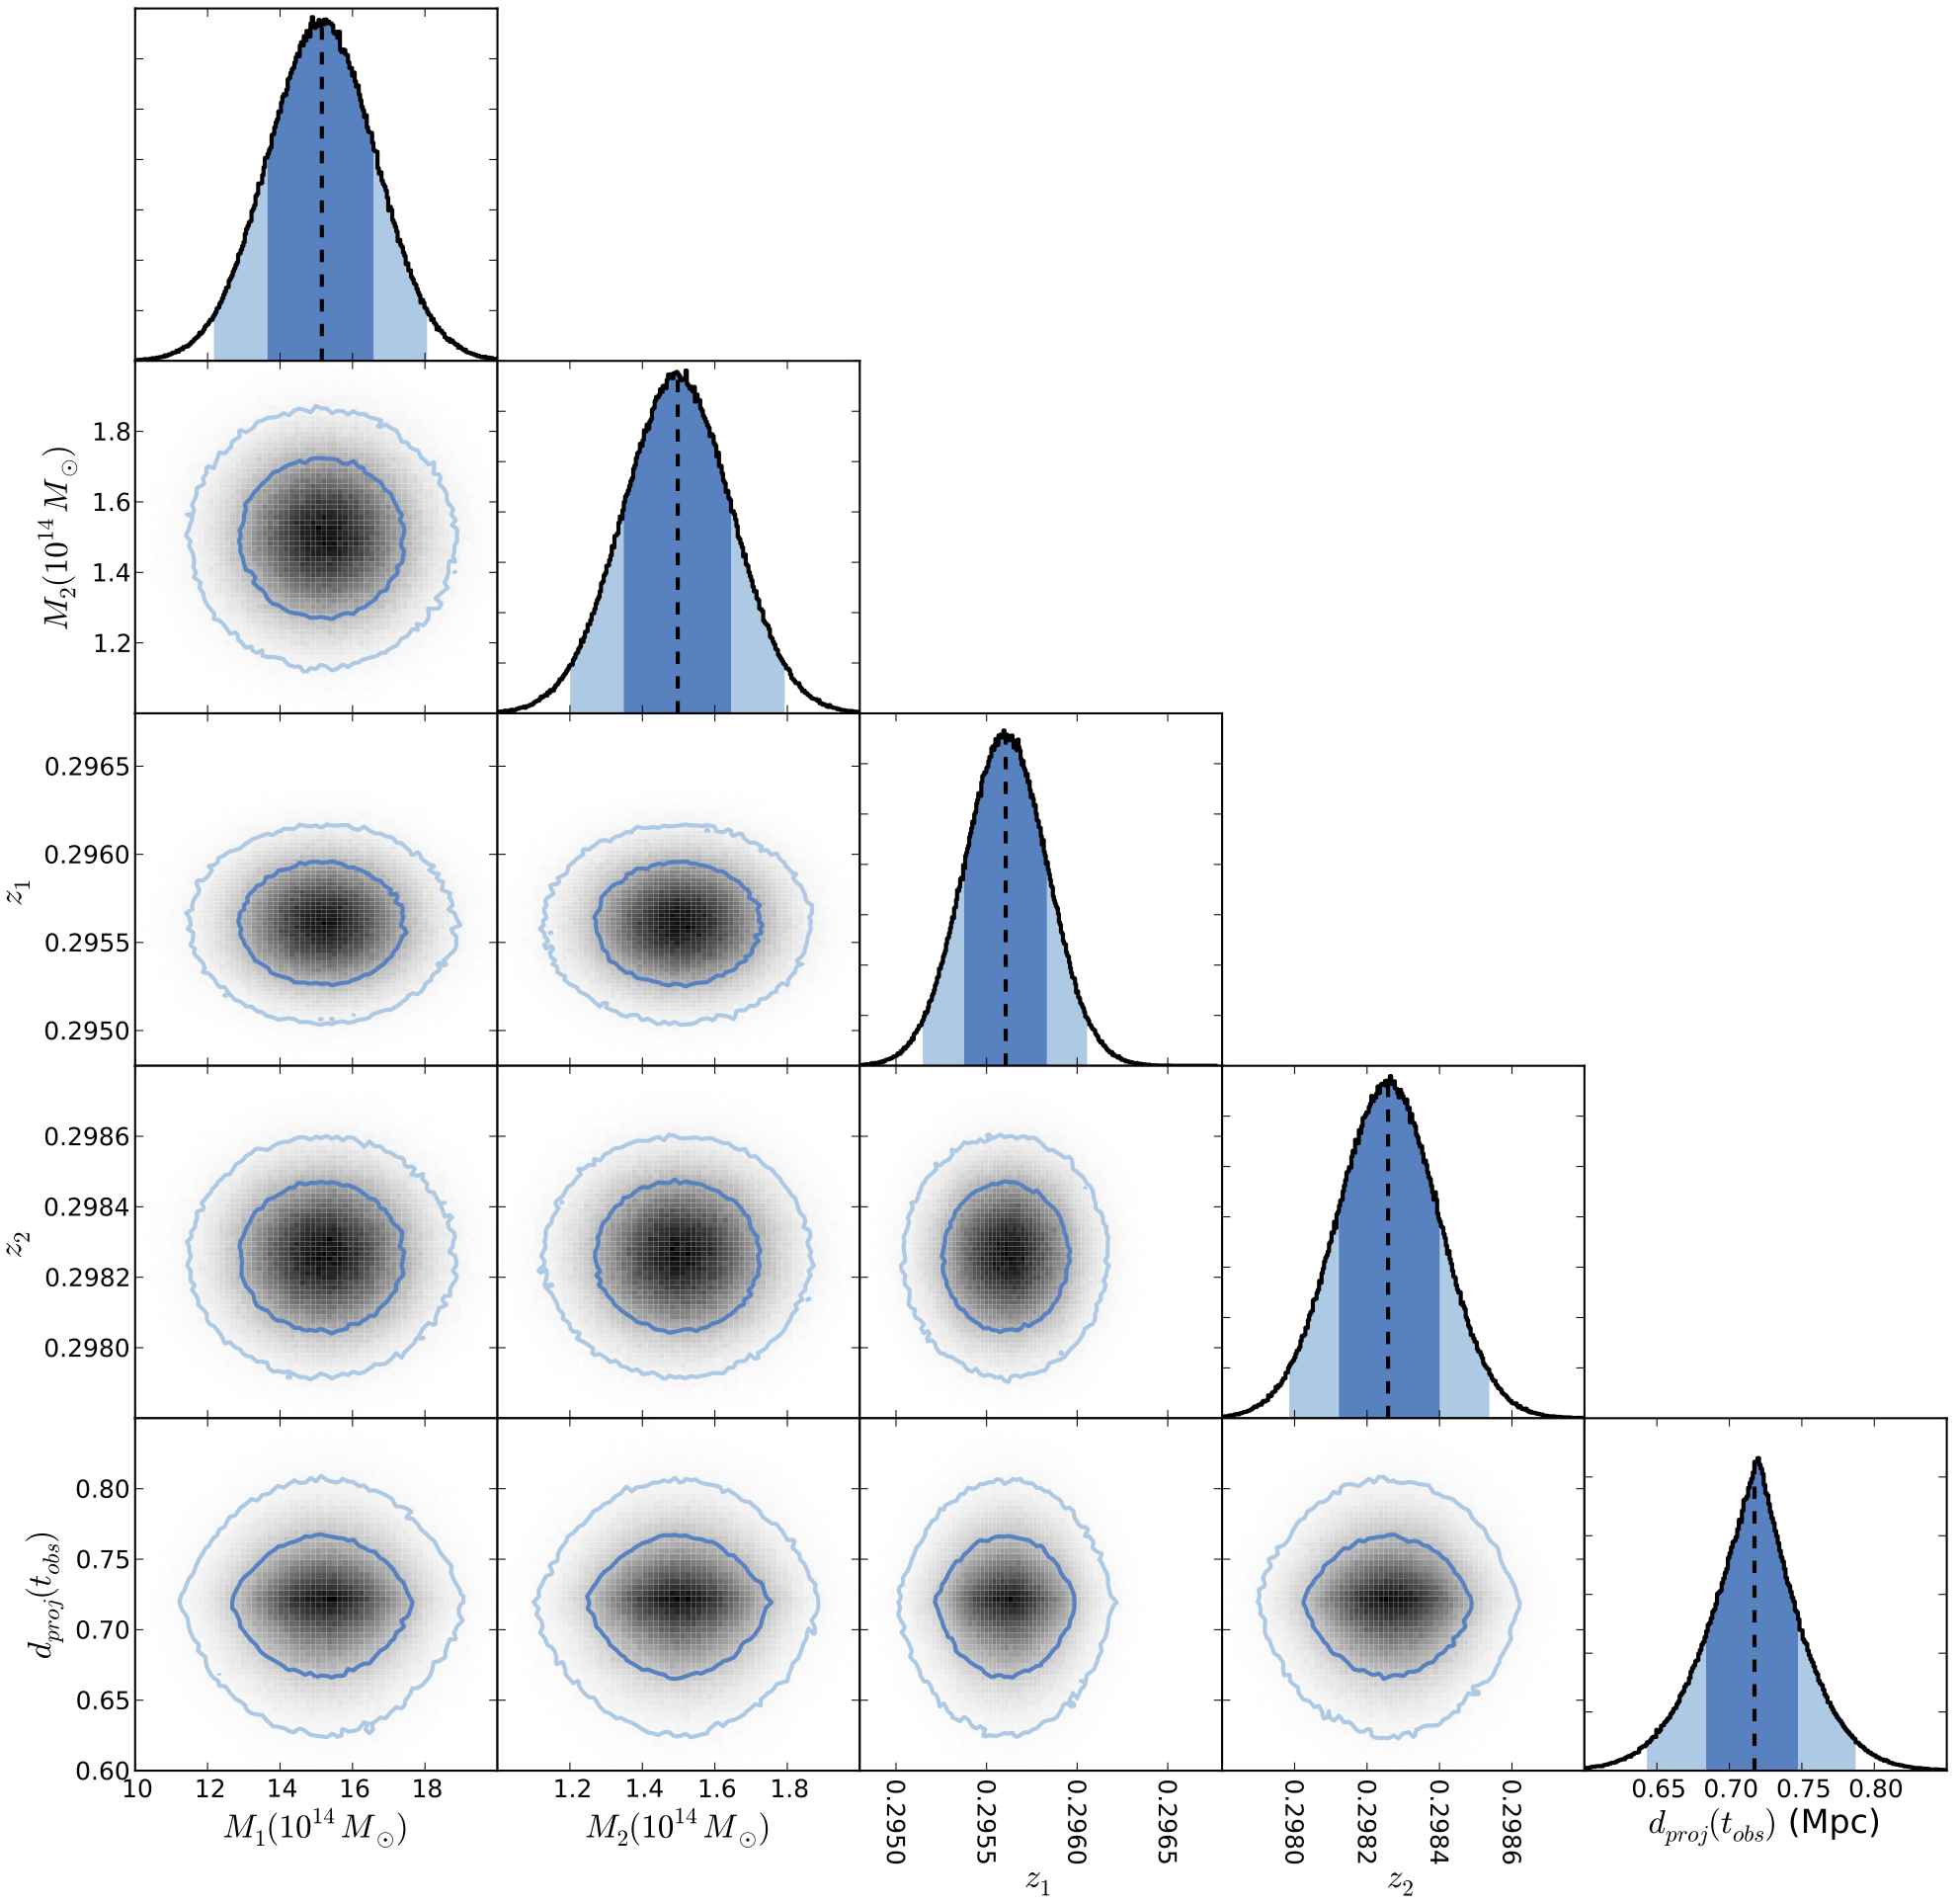
\includegraphics[width=6in]{Appendix1/bullet_shockprior_input-input.png}
\caption[Bullet Cluster marginalized \emph{Input vs.\,Input} parameters result plots.]{Bullet Cluster marginalized \emph{Input vs.\,Input} parameters result plots, for the case including the added temporal prior of \S\ref{sec_addedprior}. Dark and light blue colors correspond to 68\% and 95\% confidence intervals, respectively.  The black dashed line is the biweight-statistic location \citep{Beers:1982dp}. 
\label{fig_bc_inin}}
\end{figure}
%\clearpage

\begin{figure}
\centering
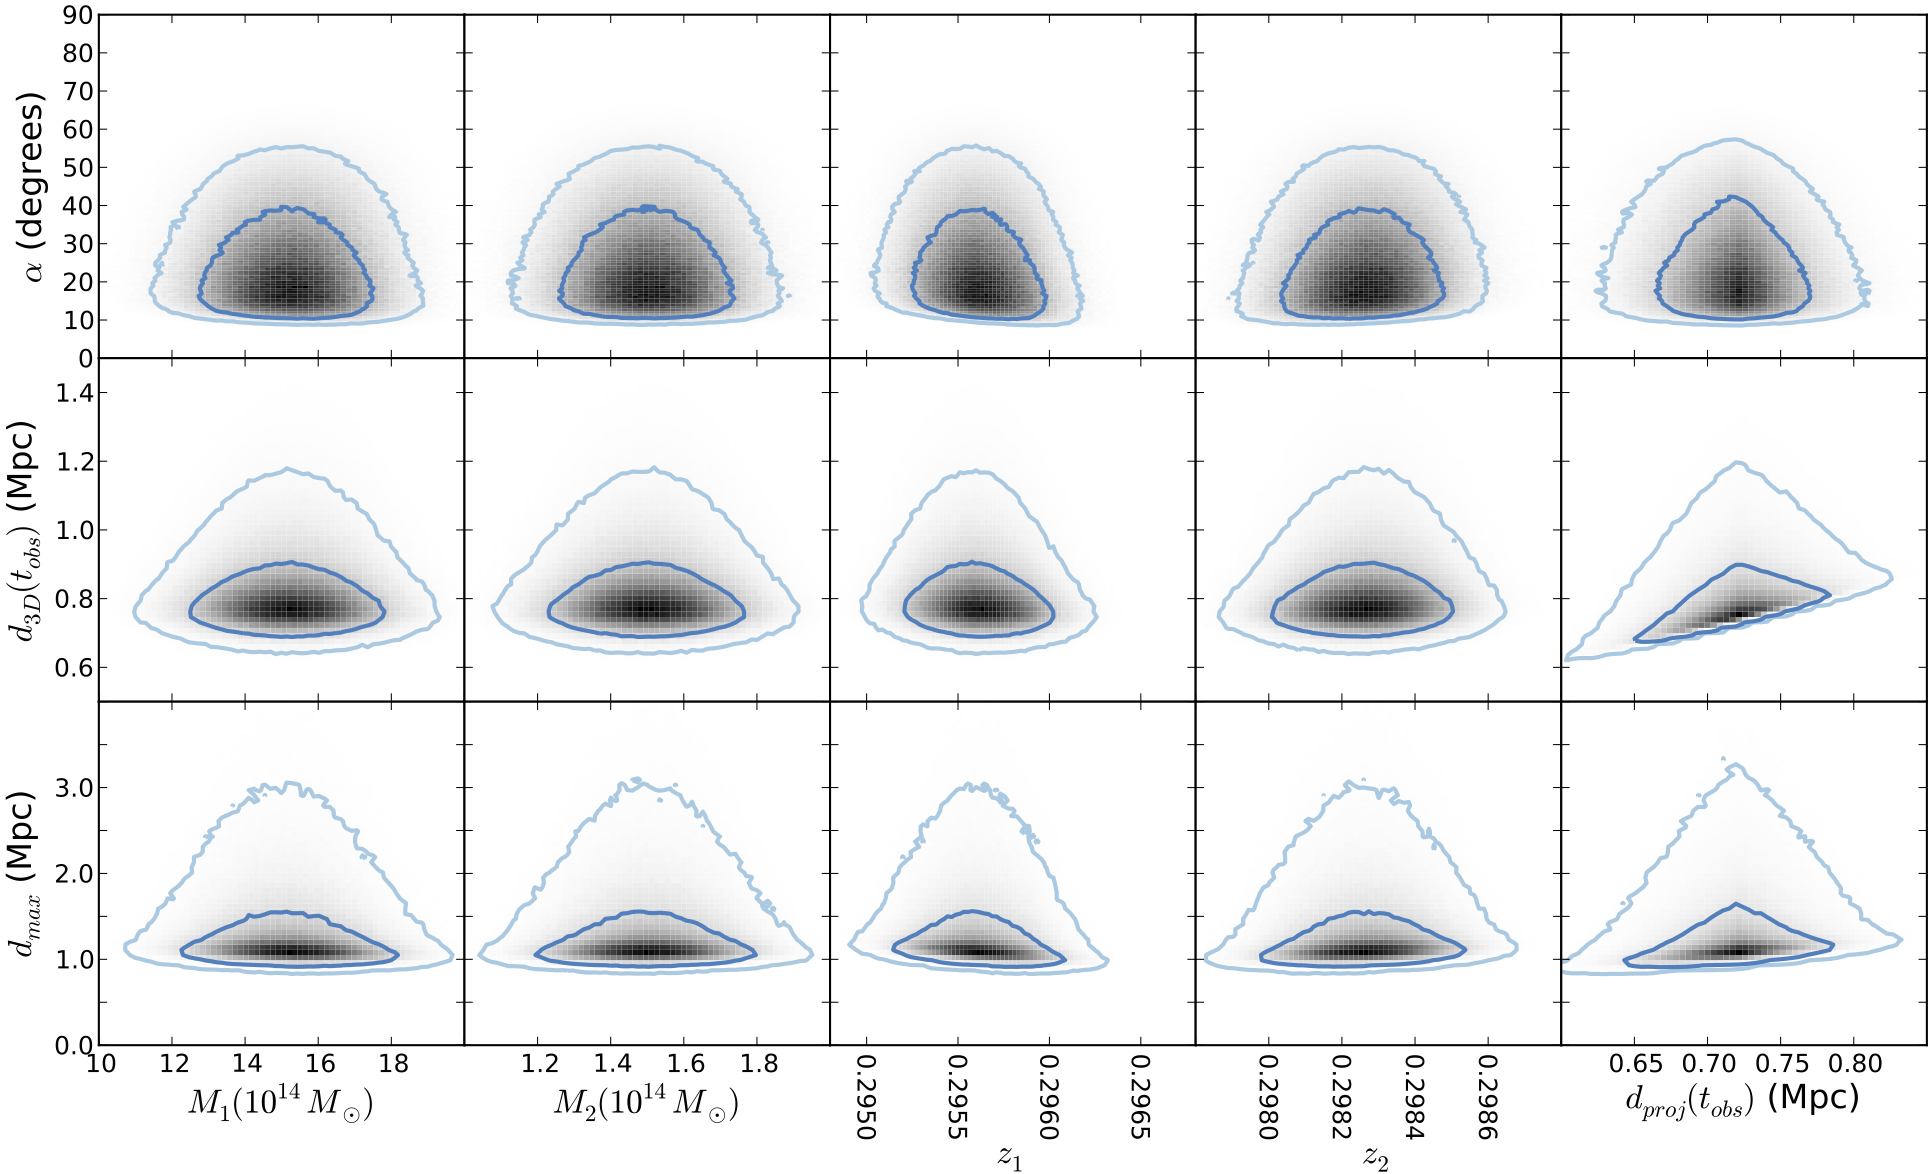
\includegraphics[width=6in]{Appendix1/bullet_shockprior_input-geometry.png}
\caption[Bullet Cluster marginalized \emph{Input vs.\,Geometry} parameters result plots.]{Bullet Cluster marginalized \emph{Input vs.\,Geometry} parameters result plots, for the case including the added temporal prior of \S\ref{sec_addedprior}.  Dark and light blue colors correspond to 68\% and 95\% confidence intervals, respectively.
\label{fig_bc_ingeo}}
\end{figure}
%\clearpage

\begin{figure}
\centering
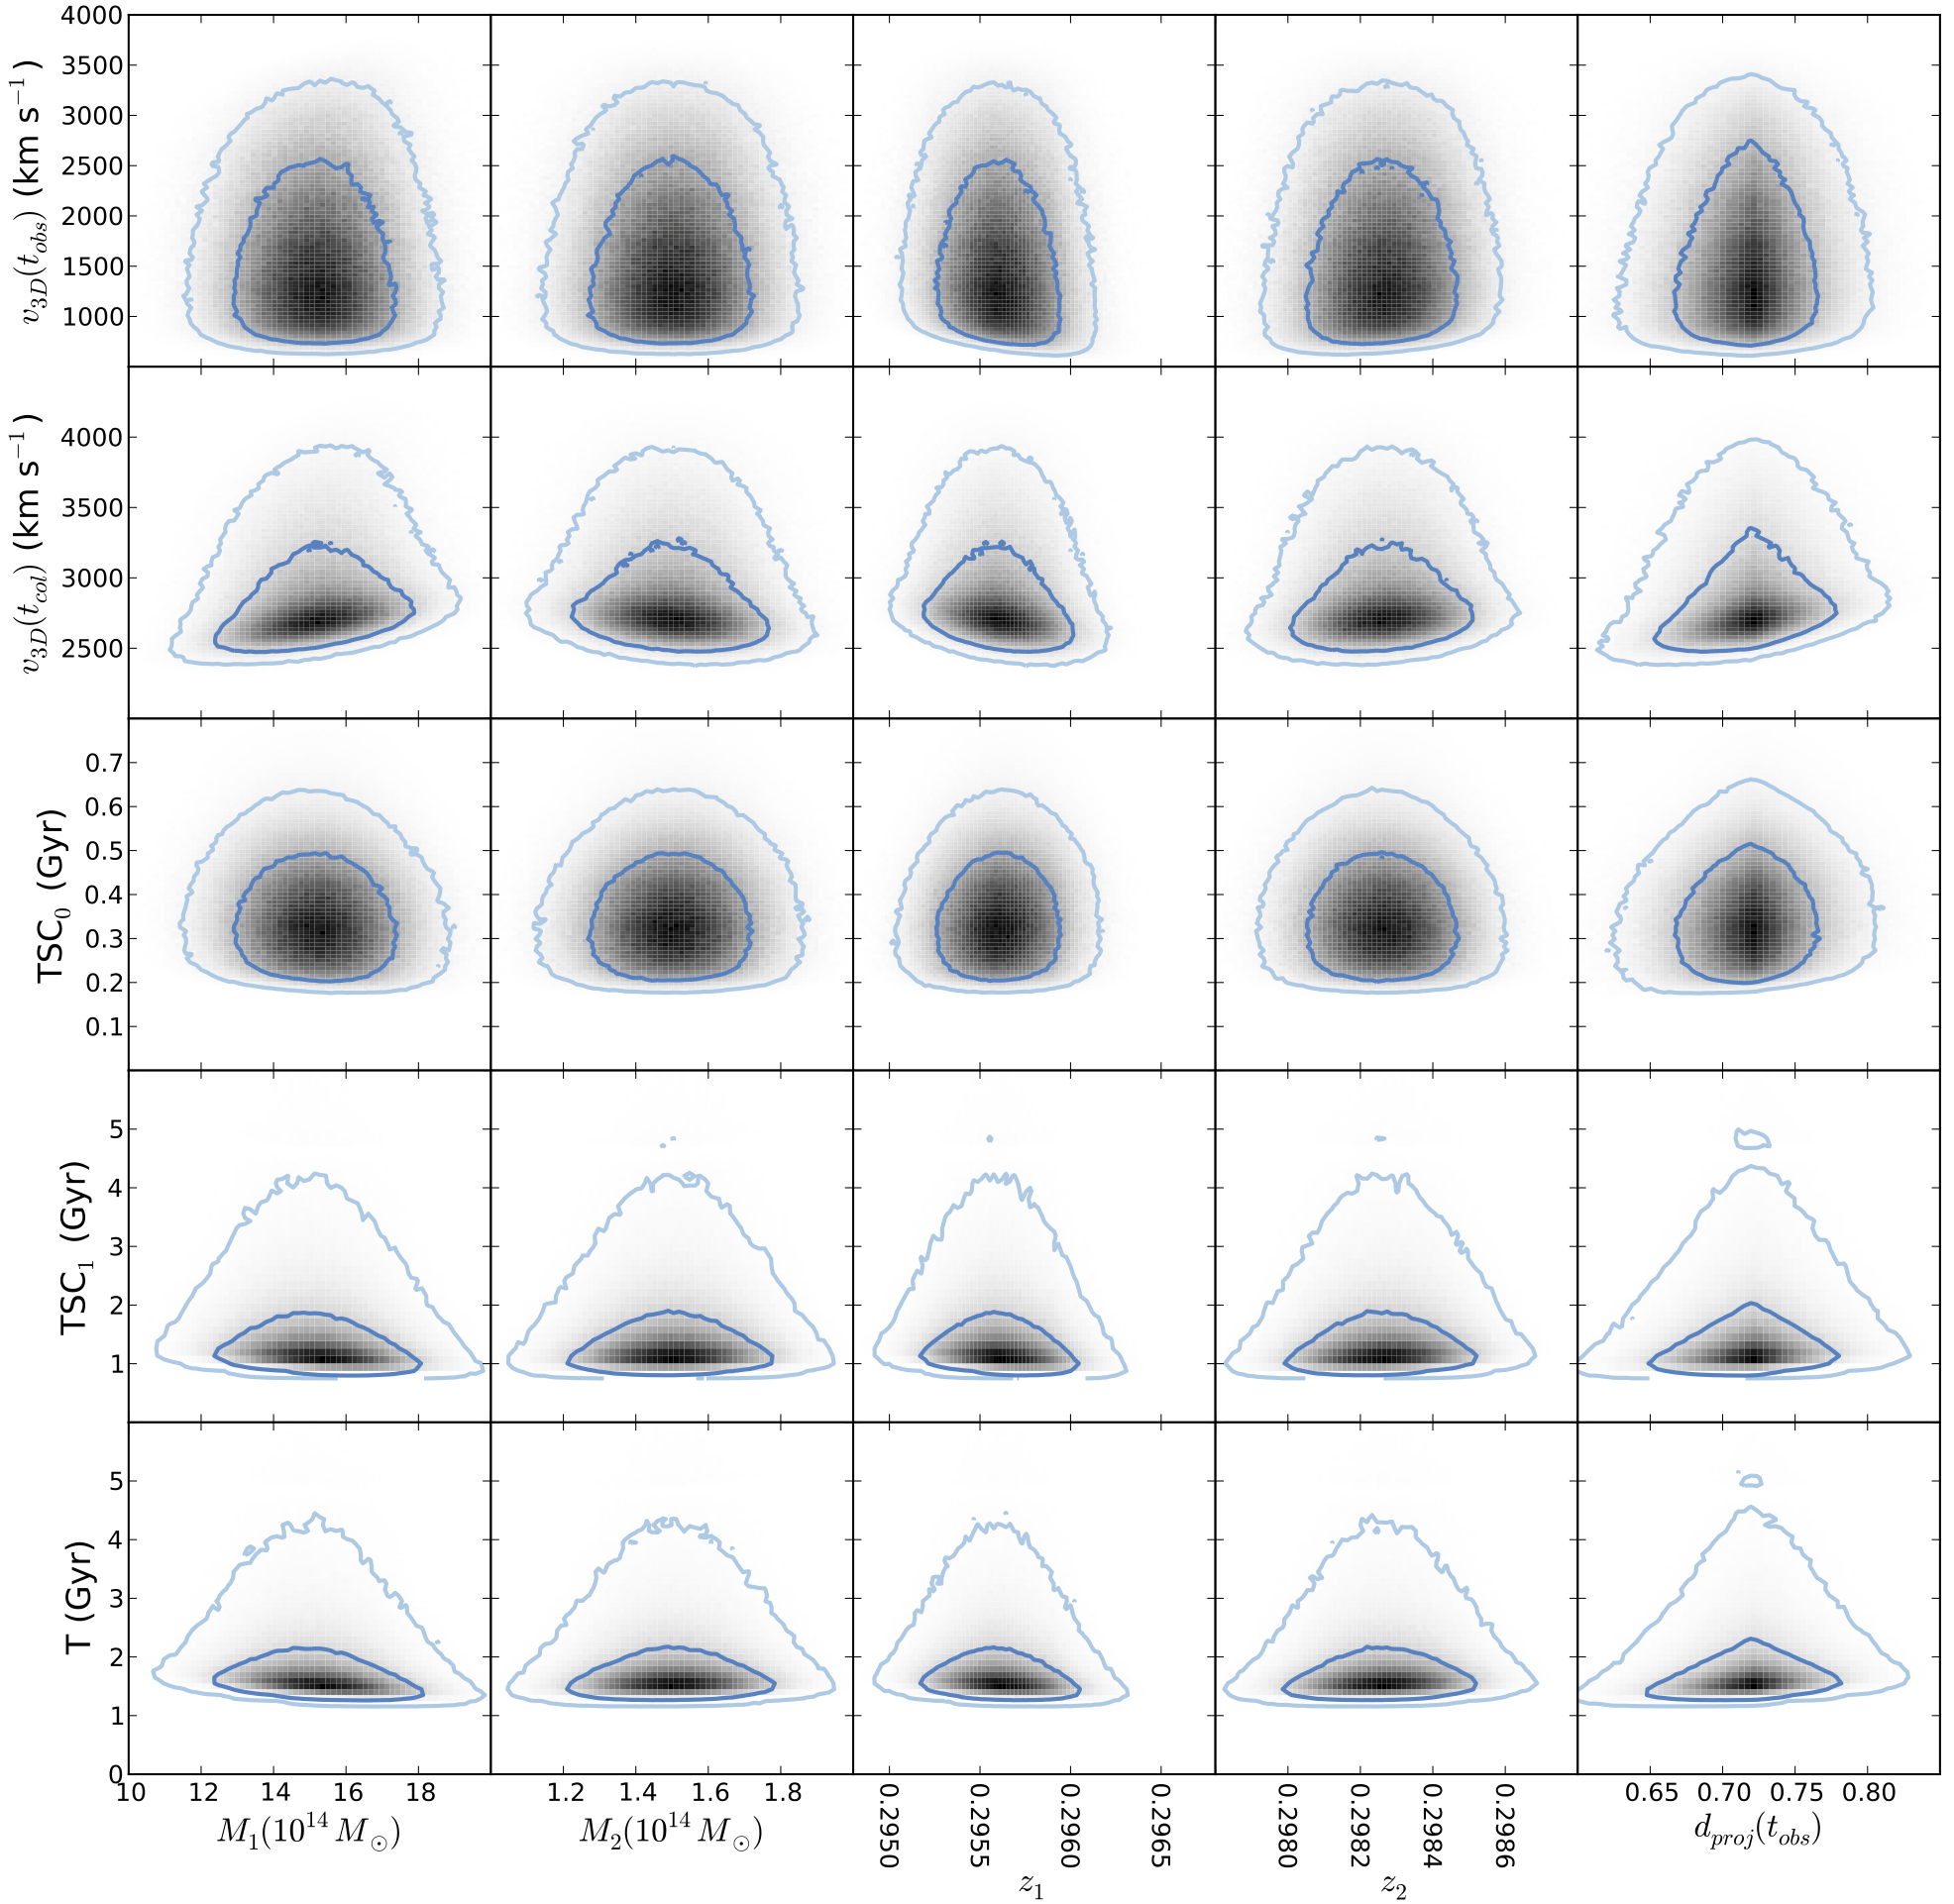
\includegraphics[width=6in]{Appendix1/bullet_shockprior_input-vt.png}
\caption[Bullet Cluster marginalized \emph{Input vs.\,Velocity \& Time} parameters result plots.]{Bullet Cluster marginalized \emph{Input vs.\,Velocity \& Time} parameters result plots, for the case including the added temporal prior of \S\ref{sec_addedprior}.  Dark and light blue colors correspond to 68\% and 95\% confidence intervals, respectively.
\label{fig_bc_invt}}
\end{figure}
%\clearpage

\begin{figure}
\centering
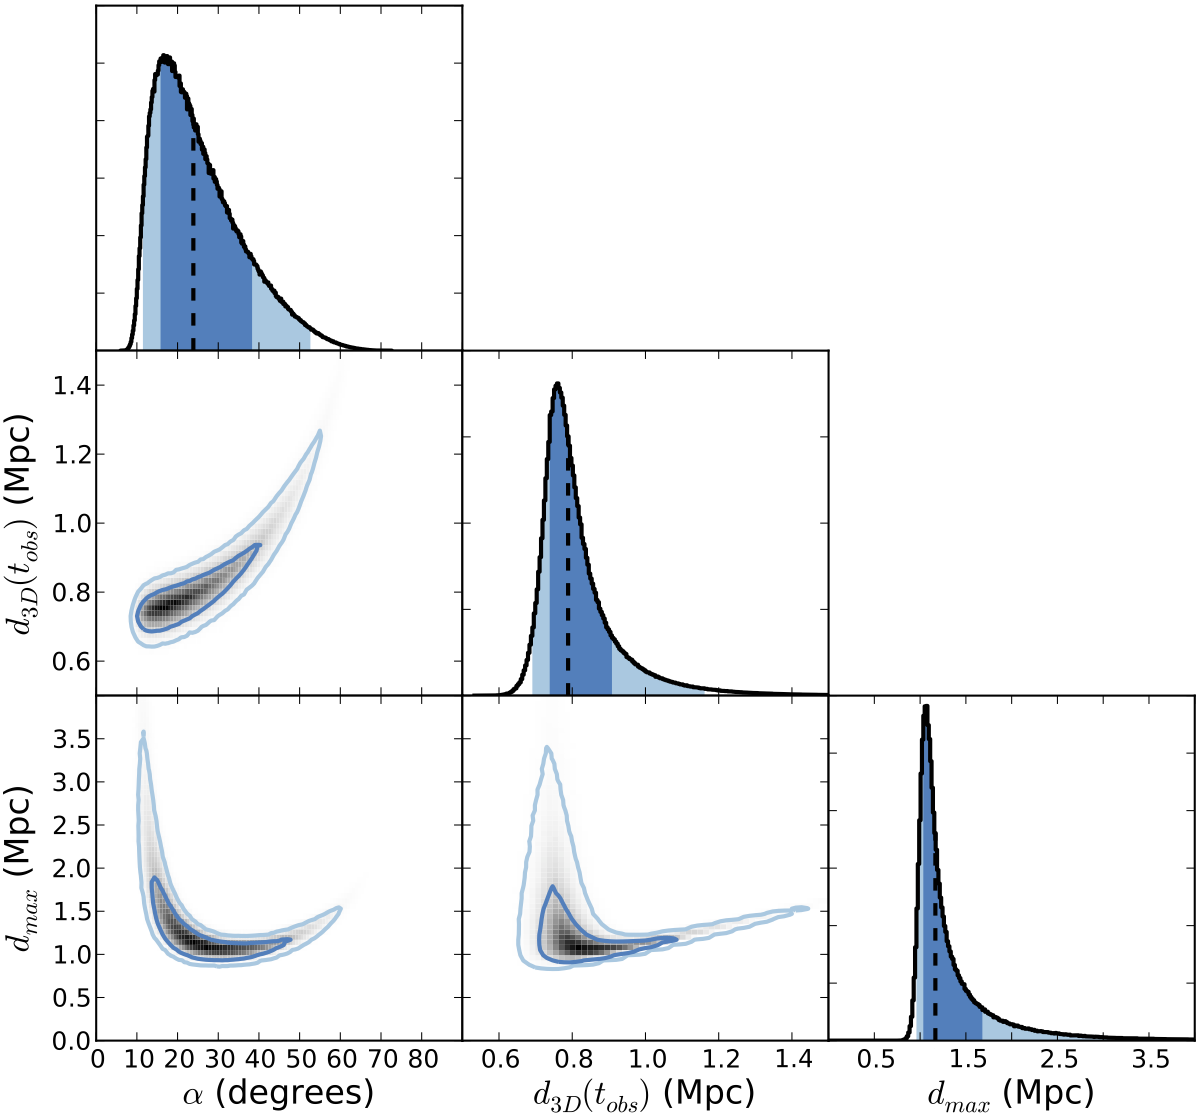
\includegraphics[width=6in]{Appendix1/bullet_shockprior_geometry-geometry.png}
\caption[Bullet Cluster marginalized \emph{Geometry vs.\,Geometry} parameters result plots.]{Bullet Cluster marginalized \emph{Geometry vs.\,Geometry} parameters result plots, for the case including the added temporal prior of \S\ref{sec_addedprior}.  Dark and light blue colors correspond to 68\% and 95\% confidence intervals, respectively.  The black dashed line is the biweight-statistic location \citep{Beers:1982dp}.
\label{fig_bc_geogeo}}
\end{figure}
%\clearpage

\begin{figure}
\centering
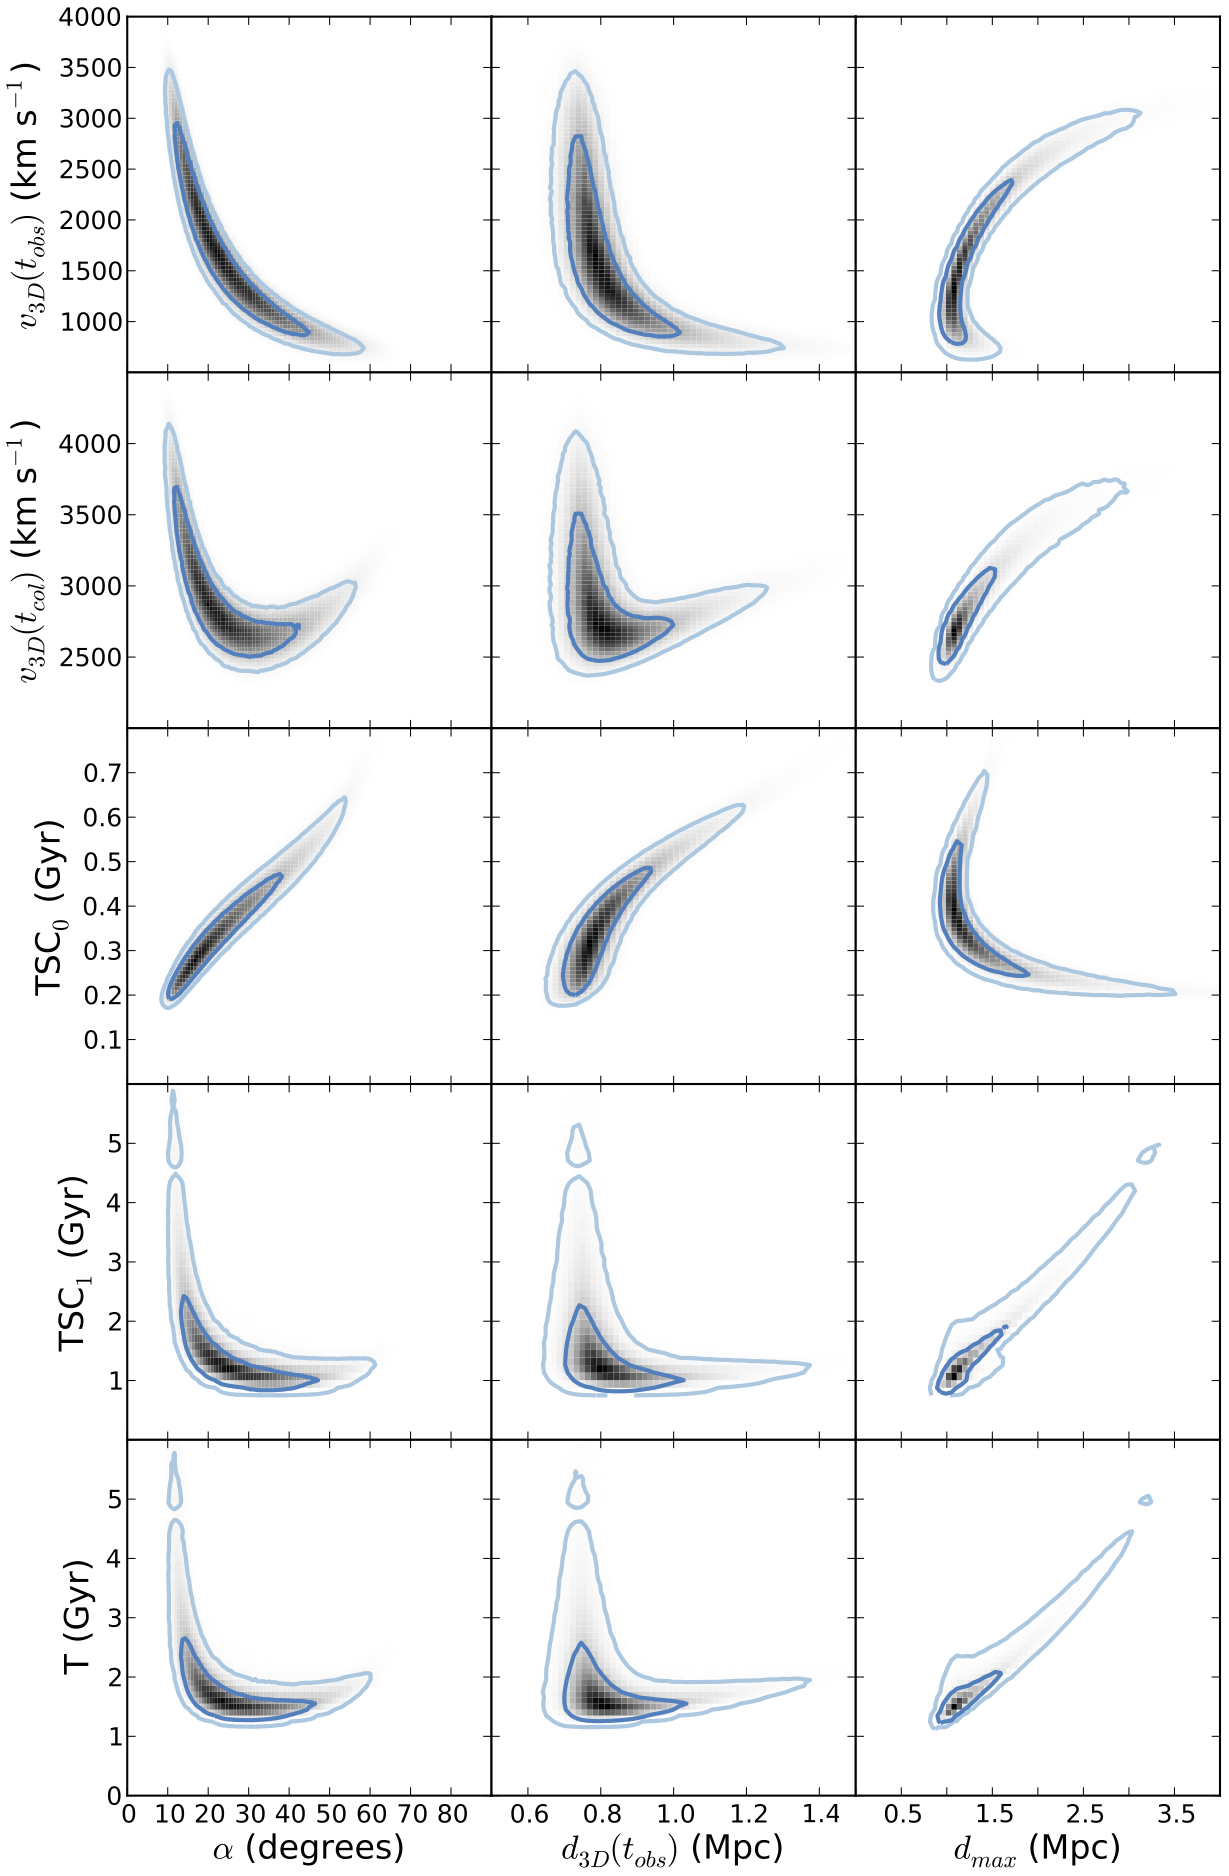
\includegraphics[height=7in]{Appendix1/bullet_shockprior_geometry-vt.png}
\caption[Bullet Cluster marginalized \emph{Geometry vs.\,Velocity \& Time} parameters result plots.]{Bullet Cluster marginalized \emph{Geometry vs.\,Velocity \& Time} parameters result plots, for the case including the added temporal prior of \S\ref{sec_addedprior}.  Dark and light blue colors correspond to 68\% and 95\% confidence intervals, respectively.
\label{fig_bc_geovt}}
\end{figure}
%\clearpage

\begin{figure}
\centering
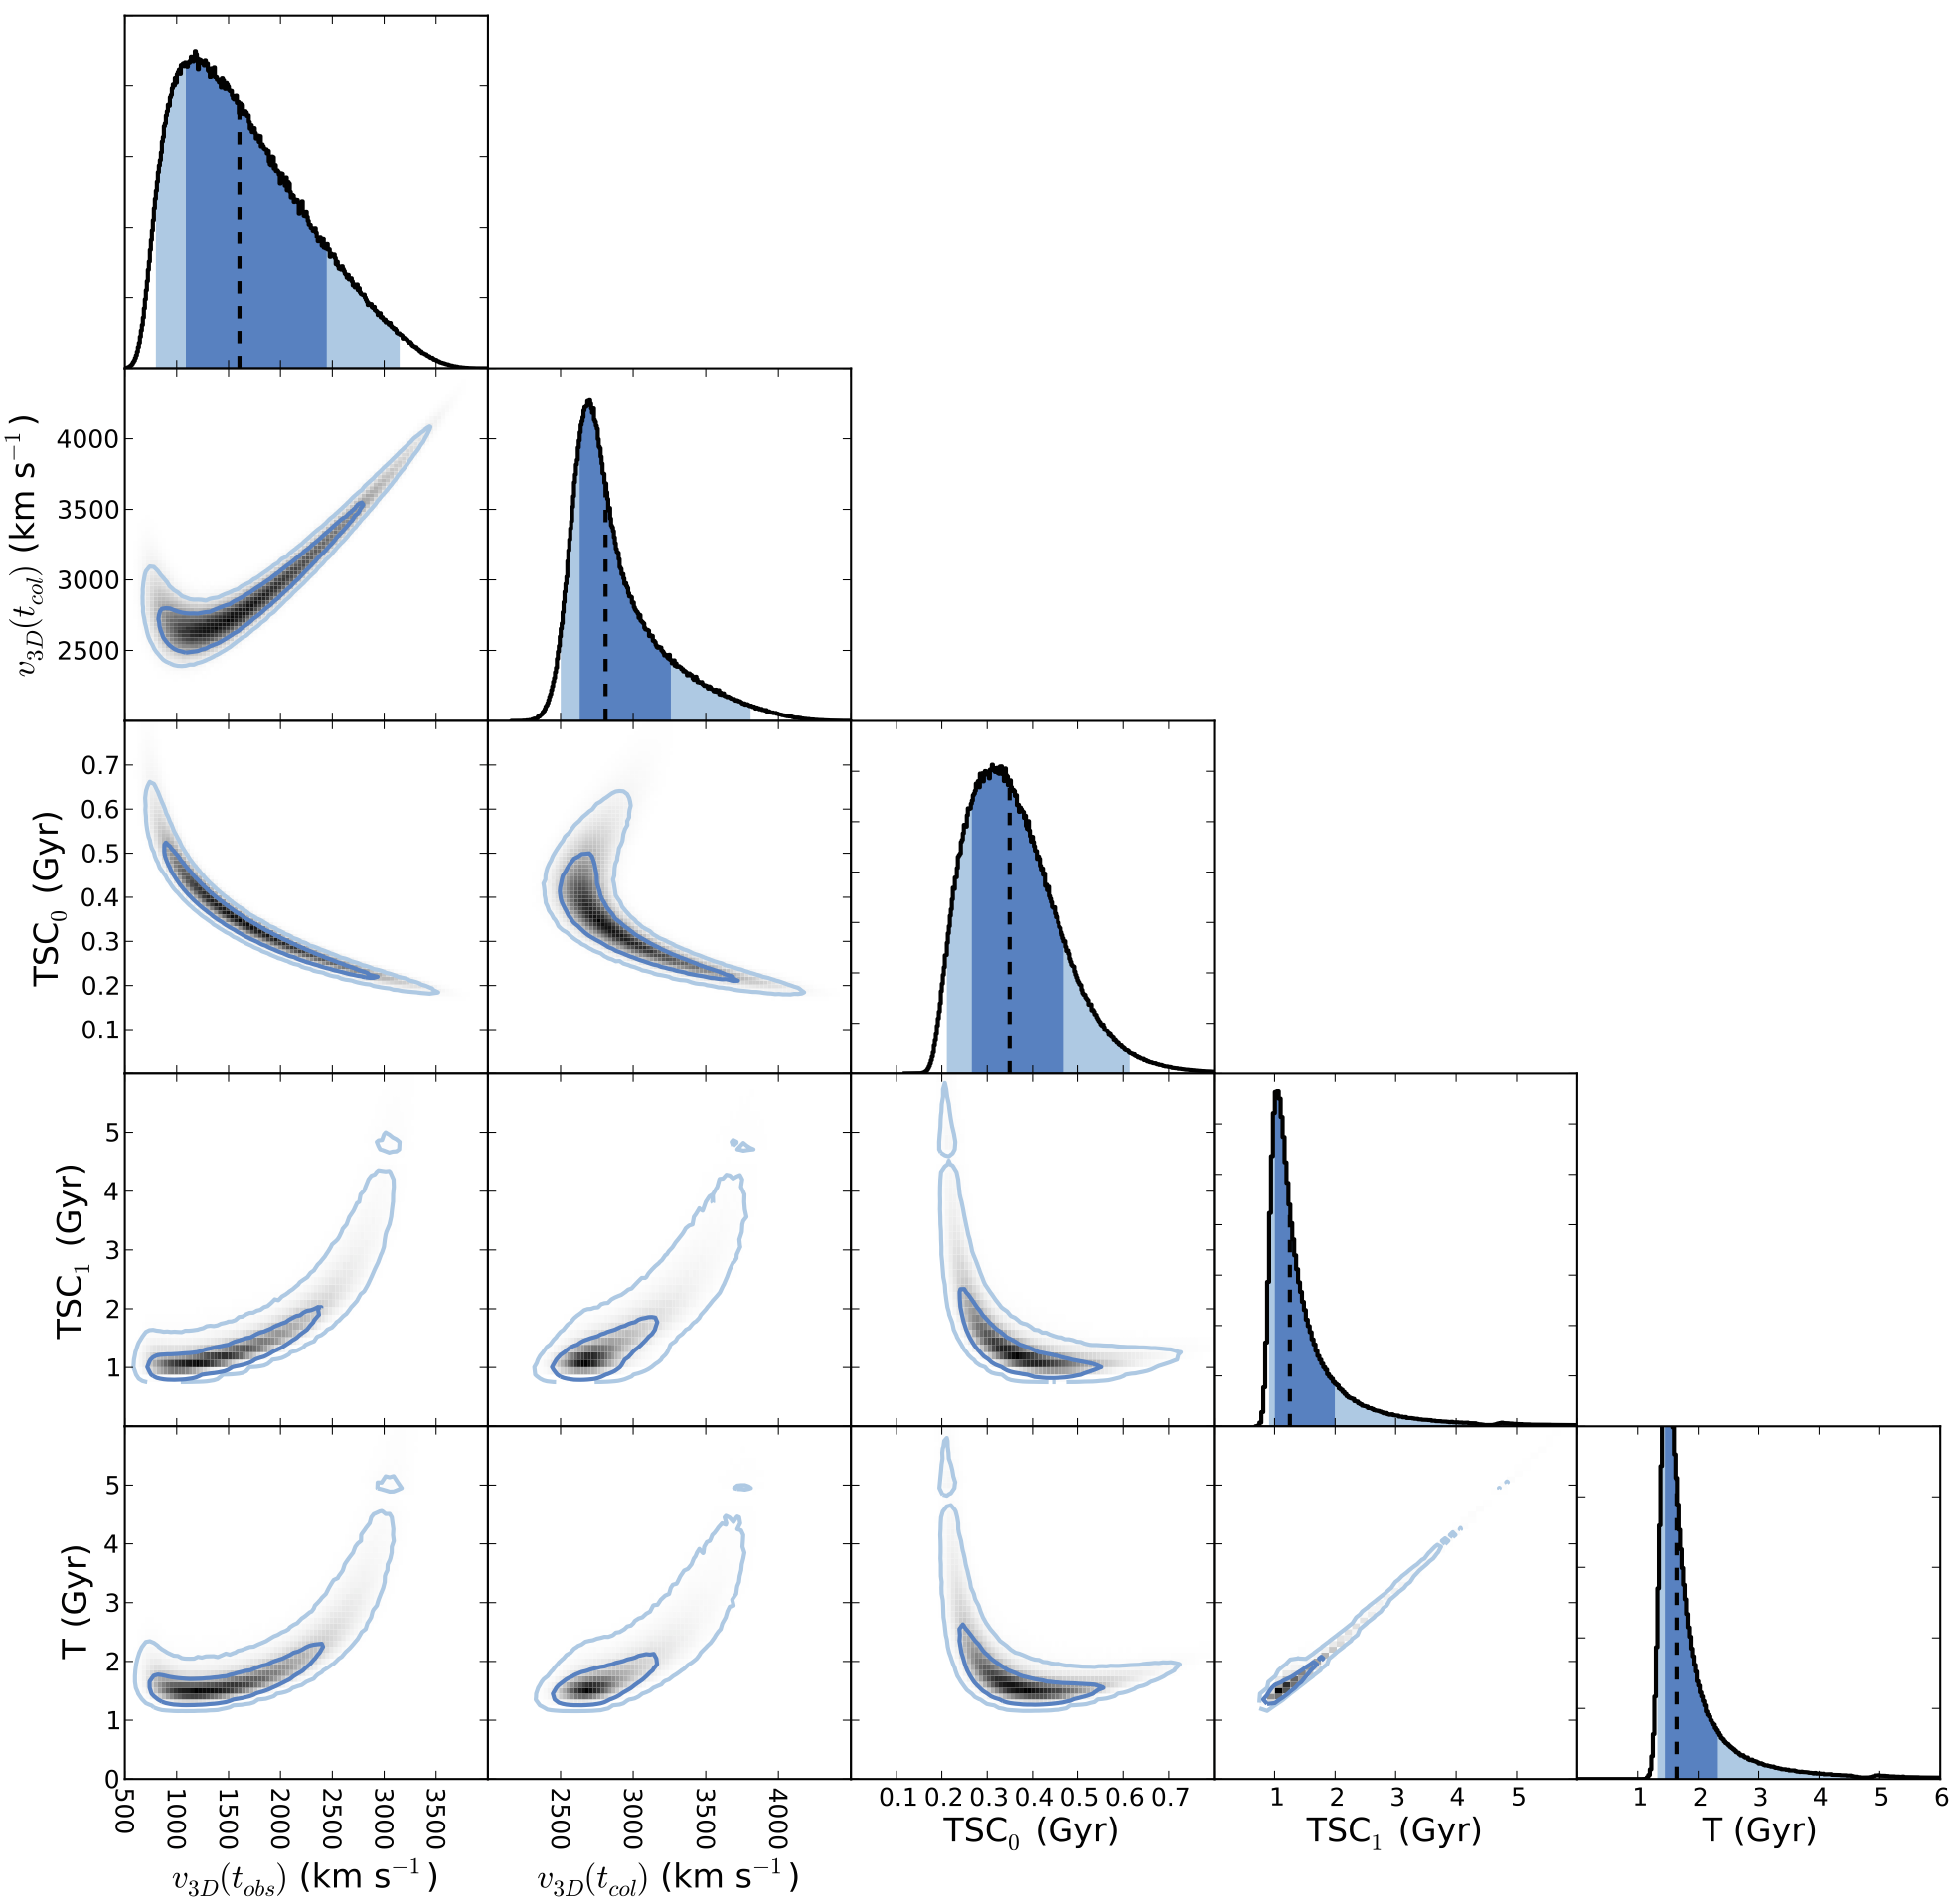
\includegraphics[width=6in]{Appendix1/bullet_shockprior_vt-vt.png}
\caption[Bullet Cluster marginalized \emph{Velocity \& Time vs.\,Velocity \& Time} parameters result plots.]{Bullet Cluster marginalized \emph{Velocity \& Time vs.\,Velocity \& Time} parameters result plots, for the case including the added temporal prior of \S\ref{sec_addedprior}.  Dark and light blue colors correspond to 68\% and 95\% confidence intervals, respectively.  The black dashed line is the biweight-statistic location \citep{Beers:1982dp}.
\label{fig_bc_vtvt}}
\end{figure}
\clearpage


\section{Musket Ball Cluster Result Plots}\label{sec_mbcresults}

This section contains the parameter results array plots for the Musket Ball Cluster.
Similar to \S\ref{sec_bcresults} the parameters are grouped in three categories (\emph{Input}, \emph{Geometry}, and \emph{Velocity \& Time}) resulting in a six subplot results array, see Figure \ref{fig_resultsarray}.
The \emph{Input} parameters consist of: M$_{200_1}$, M$_{200_2}$, $z_1$, $z_2$,	and $d_{\rm proj}$, where halo 1 refers to the ``south'' subcluster and halo 2 refers to the ``north'' subcluster.
The calculated \emph{Geometry} parameters consist of: $\alpha$, $d_{\rm 3D}$, and $d_{\rm max}$.
The calculated Velocity \& Time parameters consist of:  $v_{\rm 3D}(t_{\rm obs})$, $v_{\rm 3D}(t_{\rm col})$, $TSC_0$, $TSC_1$, and $T$.

\begin{figure}[b]
\centering
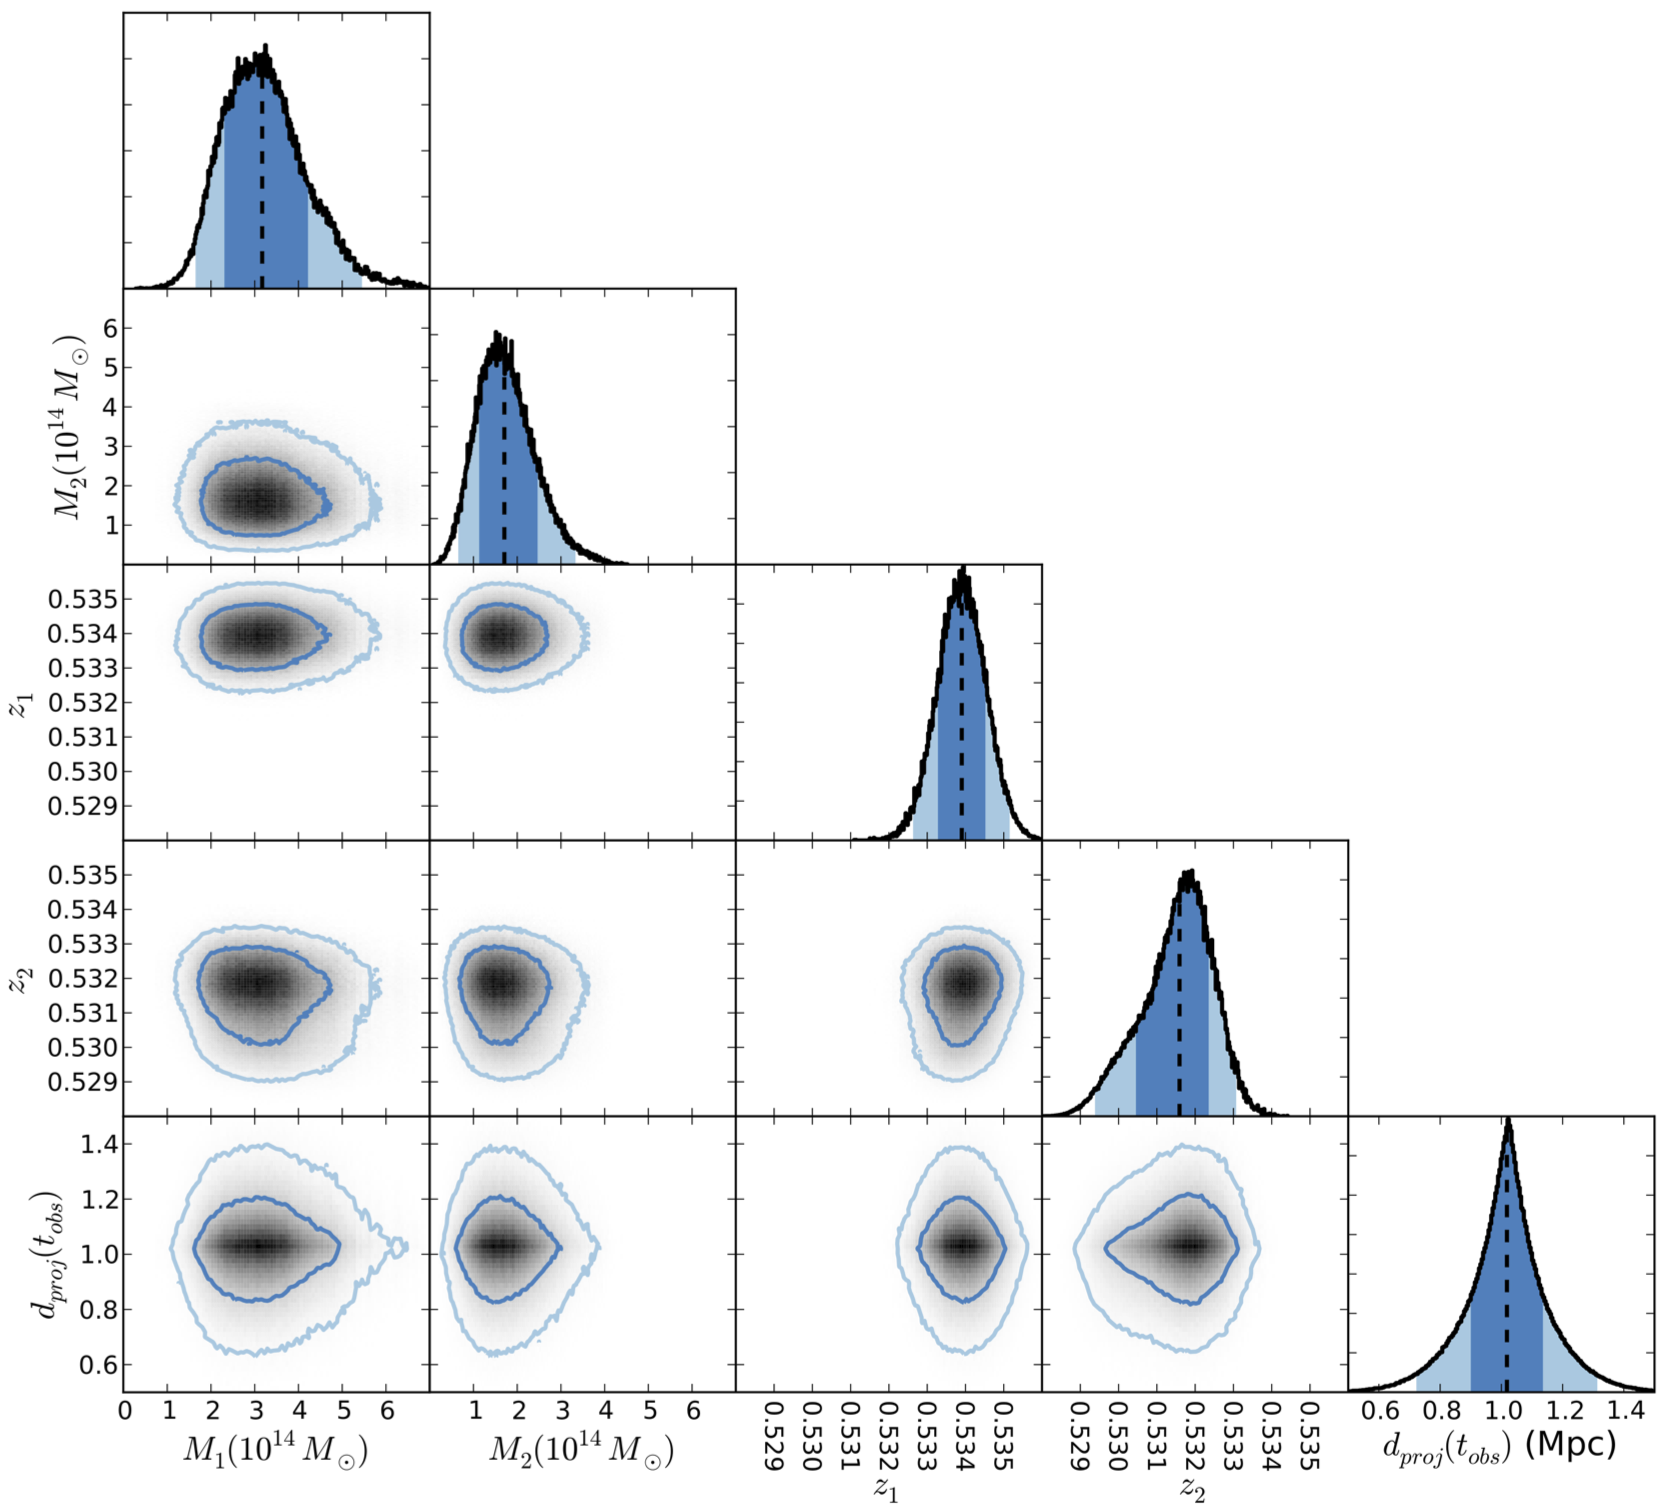
\includegraphics[width=6in]{Appendix1/run_v11_revB_input-input.png}
\caption[Musket Ball Cluster marginalized \emph{Input vs.\,Input} parameters result plots.]{Musket Ball Cluster marginalized \emph{Input vs.\,Input} parameters result plots.  Dark and light blue colors correspond to 68\% and 95\% confidence intervals, respectively.  The black dashed line is the biweight-statistic location \citep{Beers:1982dp}.
\label{musket_inin}}
\end{figure}
%\clearpage

\begin{figure}
\centering
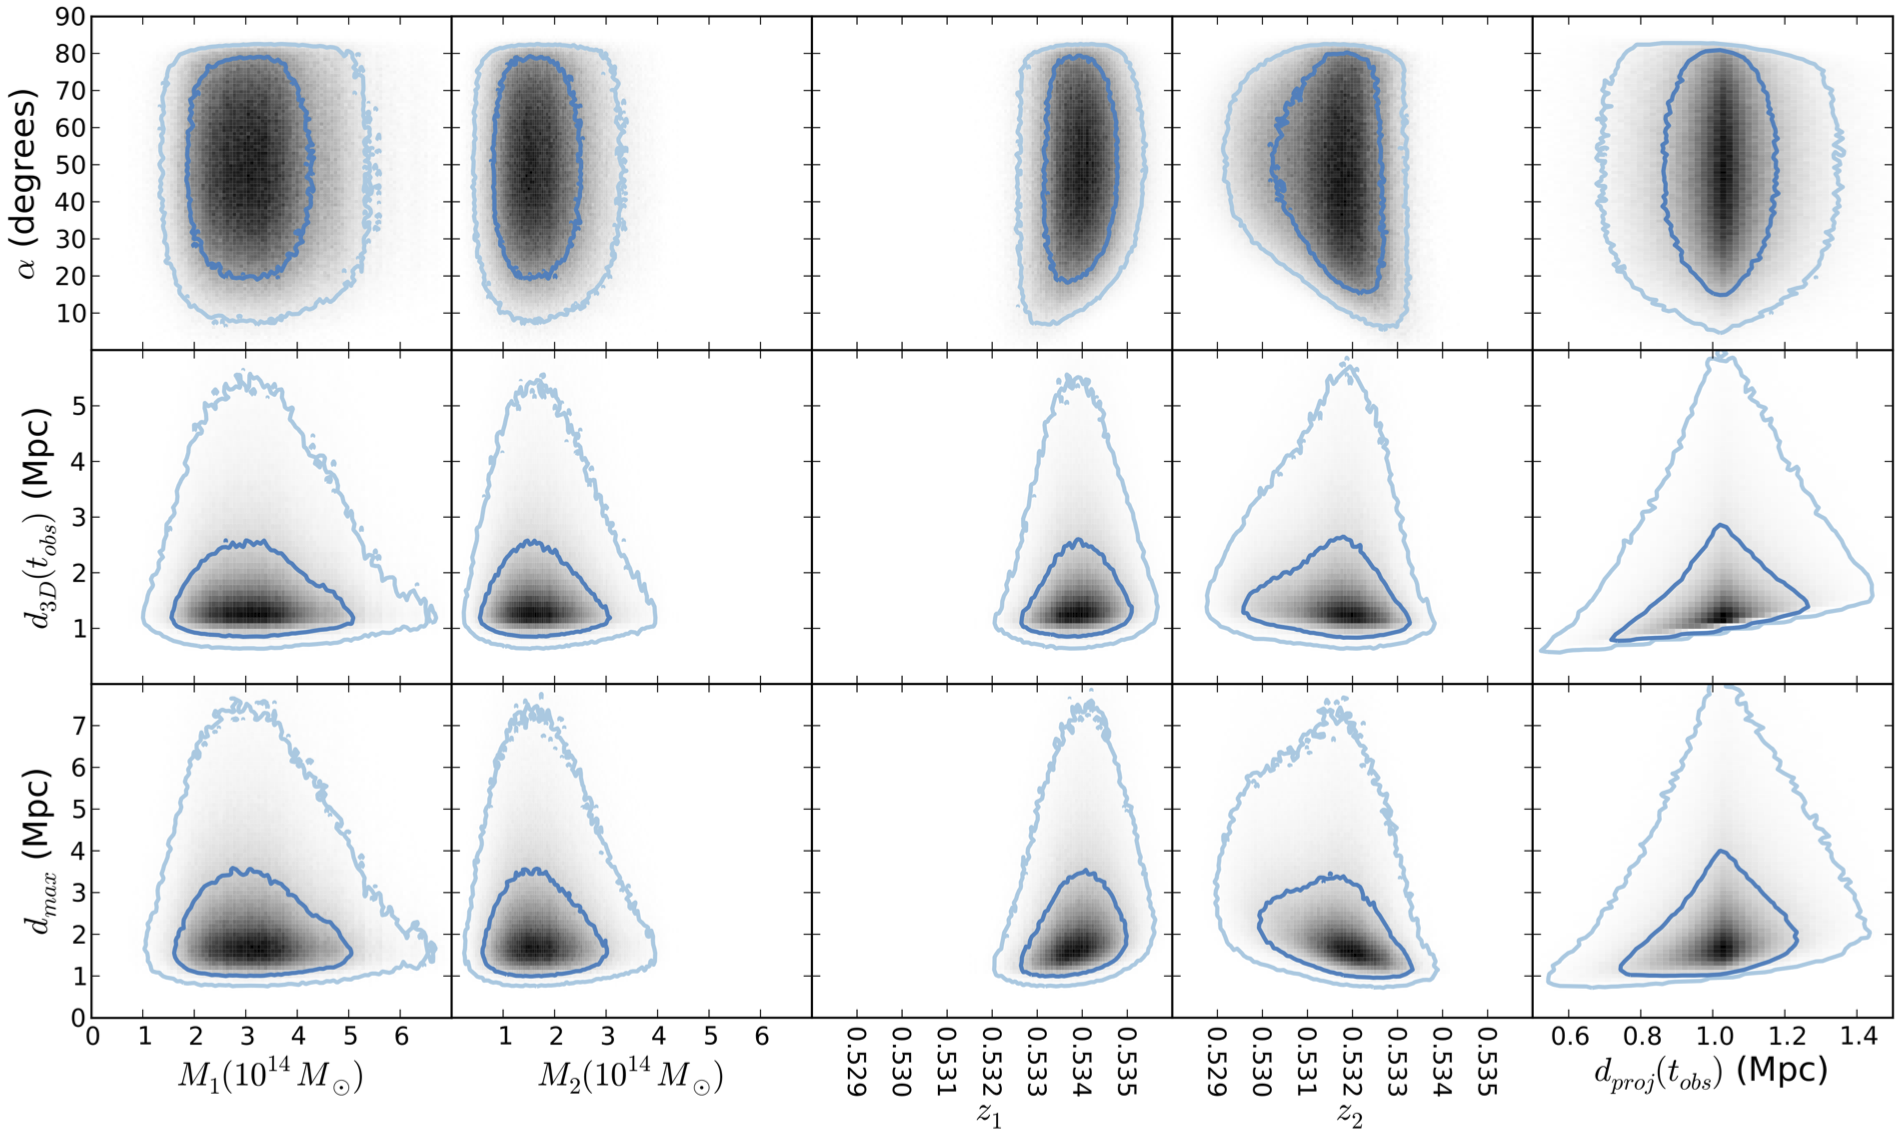
\includegraphics[width=6in]{Appendix1/run_v11_revB_input-geometry.png}
\caption[Musket Ball Cluster marginalized \emph{Input vs.\,Geometry} parameters result plots.]{Musket Ball Cluster marginalized \emph{Input vs.\,Geometry} parameters result plots.  Dark and light blue colors correspond to 68\% and 95\% confidence intervals, respectively.
\label{musket_ingeo}}
\end{figure}
%\clearpage

\begin{figure}
\centering
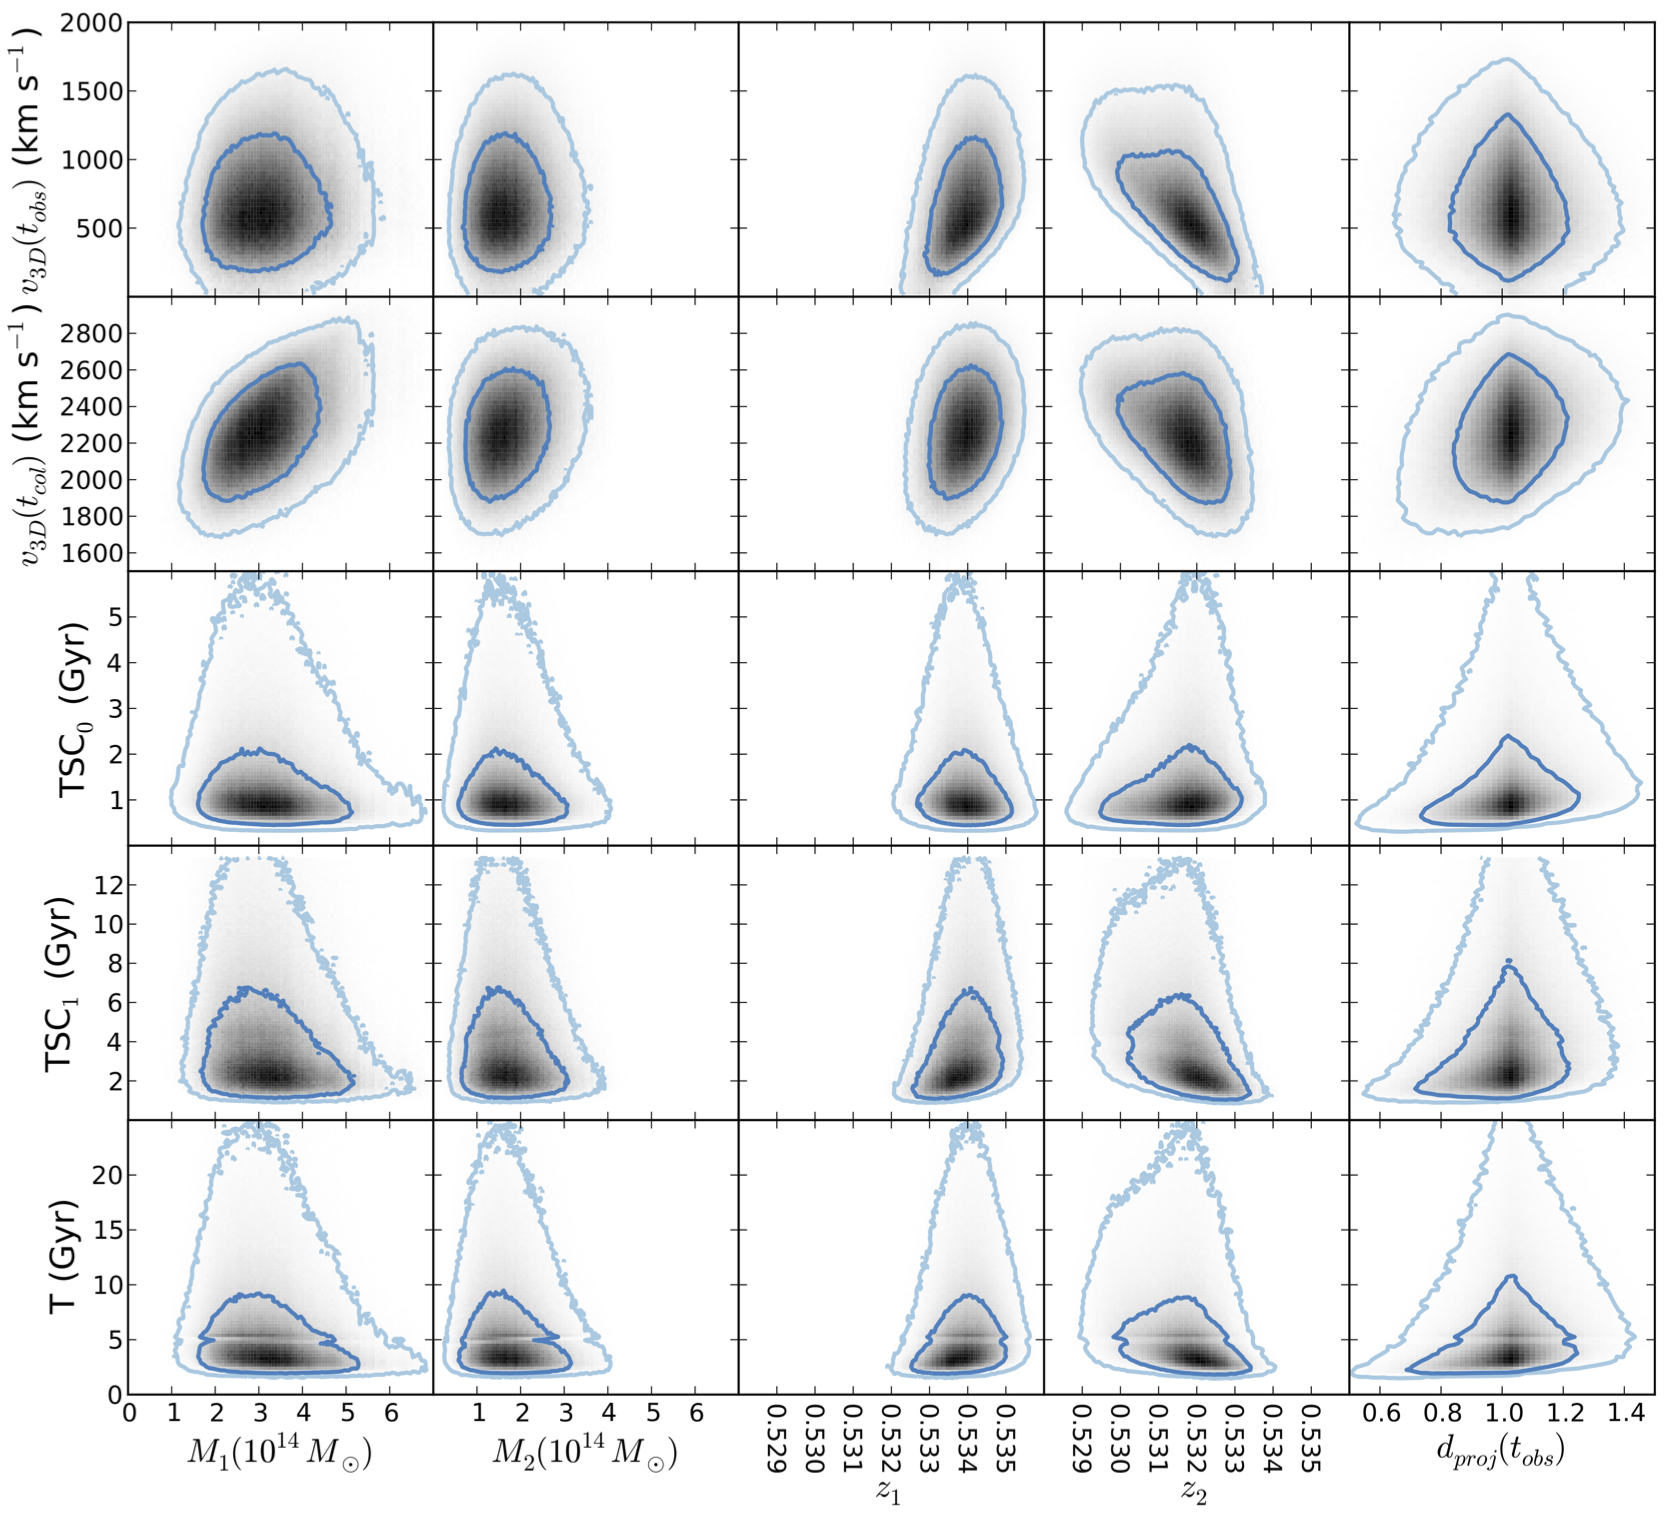
\includegraphics[width=6in]{Appendix1/run_v11_revB_input-vt.png}
\caption[Musket Ball Cluster marginalized \emph{Input vs.\,Velocity \& Time} parameters result plots.]{Musket Ball Cluster marginalized \emph{Input vs.\,Velocity \& Time} parameters result plots.  Dark and light blue colors correspond to 68\% and 95\% confidence intervals, respectively.
\label{musket_invt}}
\end{figure}
%\clearpage

\begin{figure}
\centering
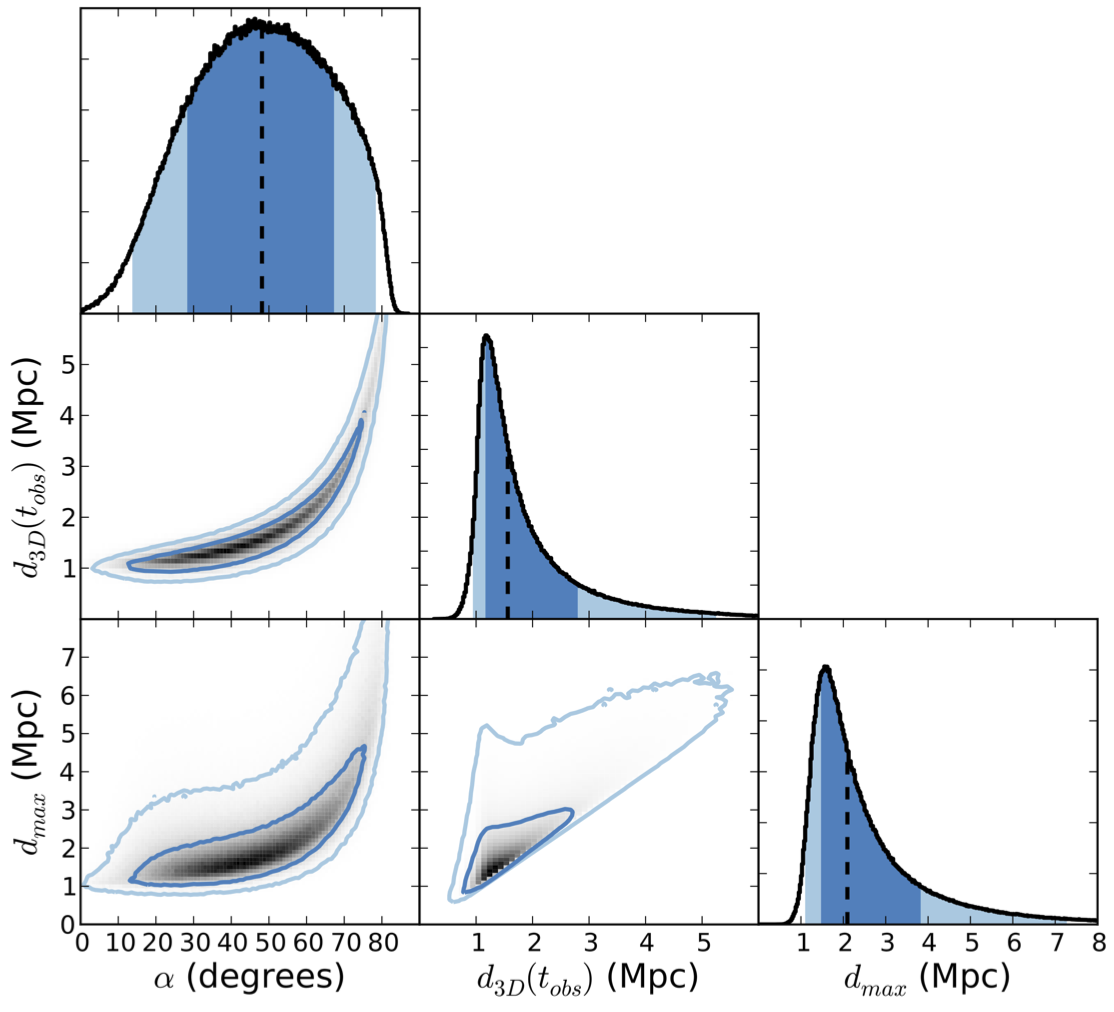
\includegraphics[width=6in]{Appendix1/run_v11_revB_geometry-geometry.png}
\caption[Musket Ball Cluster marginalized \emph{Geometry vs.\,Geometry} parameters result plots.]{Musket Ball Cluster marginalized \emph{Geometry vs.\,Geometry} parameters result plots.  Dark and light blue colors correspond to 68\% and 95\% confidence intervals, respectively.  The black dashed line is the biweight-statistic location \citep{Beers:1982dp}.
\label{musket_geogeo}}
\end{figure}
%\clearpage

\begin{figure}
\centering
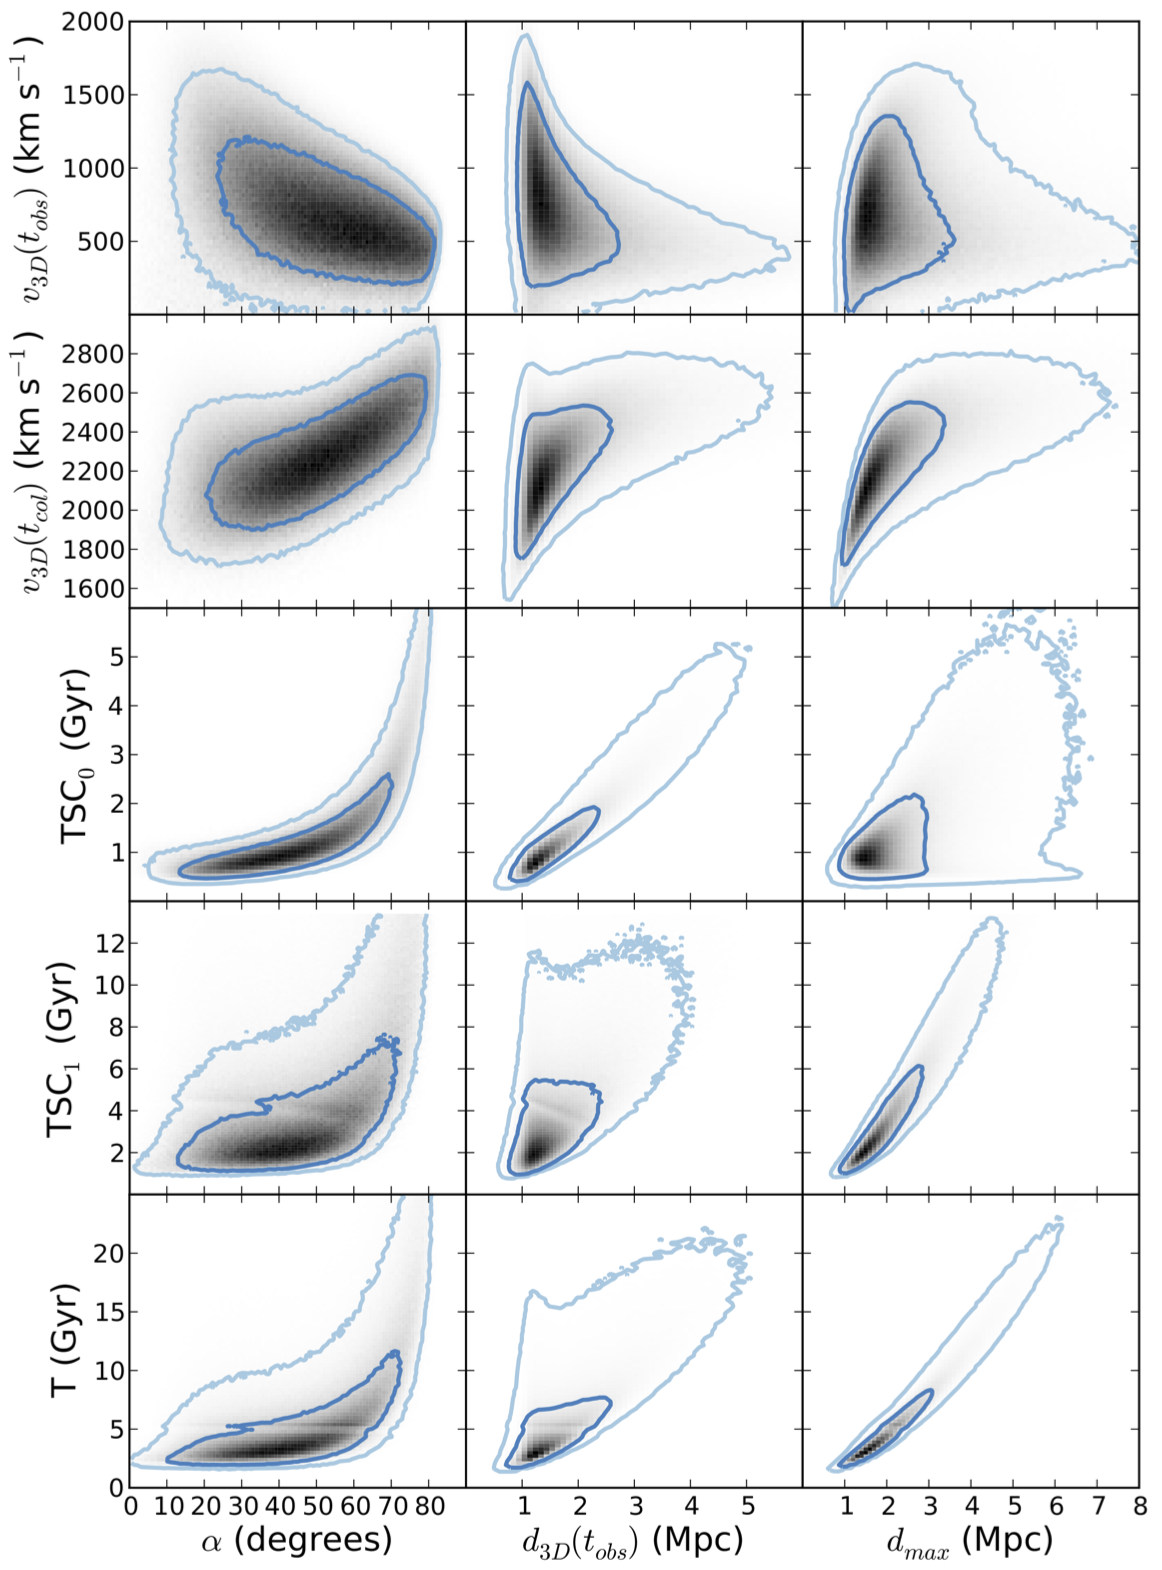
\includegraphics[height=7in]{Appendix1/run_v11_revB_geometry-vt.png}
\caption[Musket Ball Cluster marginalized \emph{Geometry vs.\,Velocity \& Time} parameters result plots.]{Musket Ball Cluster marginalized \emph{Geometry vs.\,Velocity \& Time} parameters result plots.  Dark and light blue colors correspond to 68\% and 95\% confidence intervals, respectively.
\label{musket_geovt}}
\end{figure}
%\clearpage

\begin{figure}
\centering
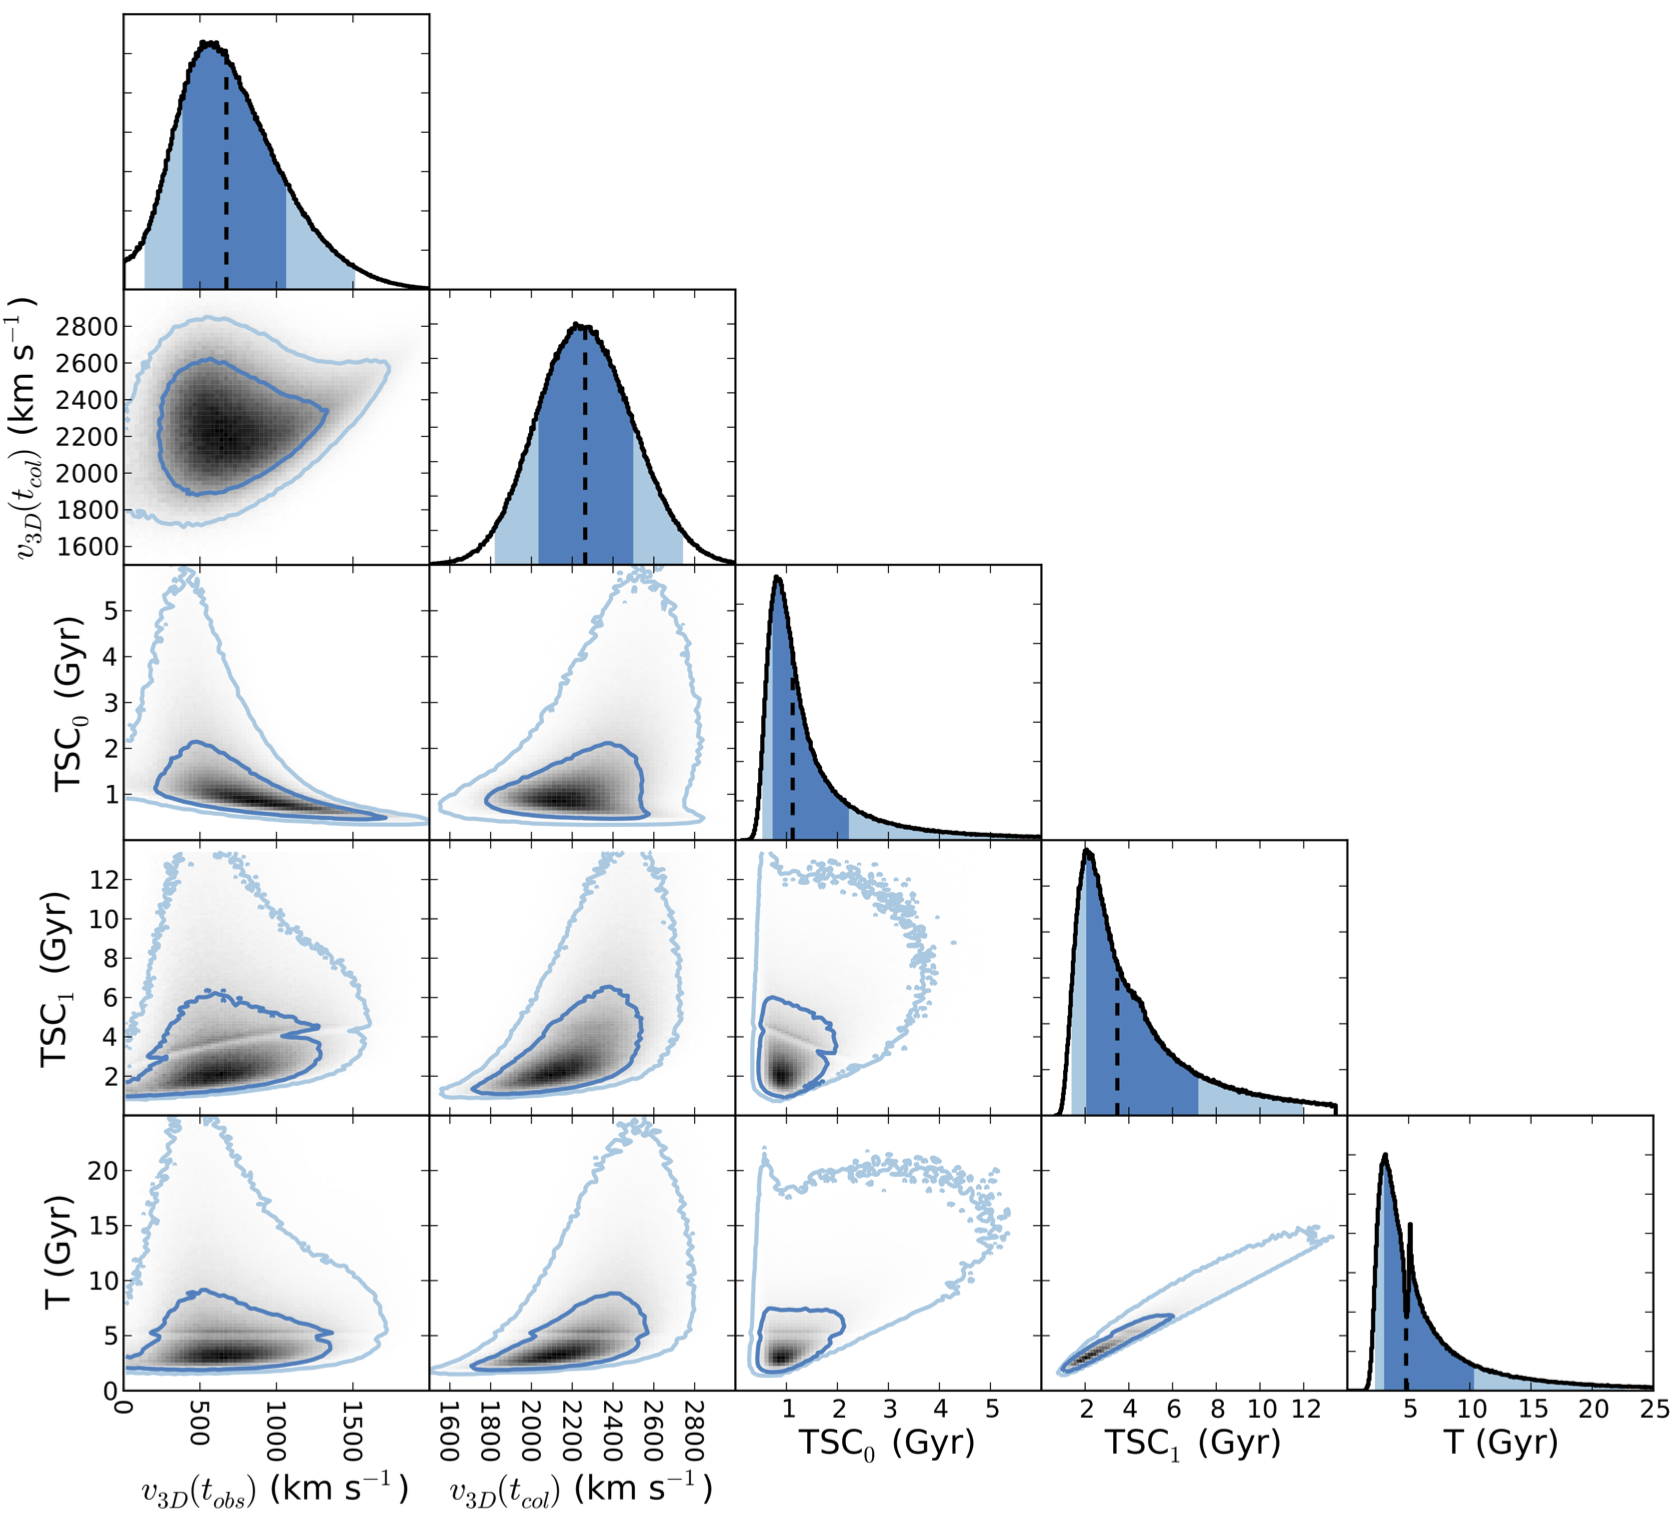
\includegraphics[width=6in]{Appendix1/run_v11_revB_vt-vt.png}
\caption[Musket Ball Cluster marginalized \emph{Velocity \& Time vs.\,Velocity \& Time} parameters result plots.]{Musket Ball Cluster marginalized \emph{Velocity \& Time vs.\,Velocity \& Time} parameters result plots.  Dark and light blue colors correspond to 68\% and 95\% confidence intervals, respectively.  The black dashed line is the biweight-statistic location \citep{Beers:1982dp}.
\label{musket_vtvt}}
\end{figure}